\documentclass[a4paper,10pt]{article}
\usepackage[margin=0.8in]{geometry}
\usepackage{enumitem}
\usepackage{hyperref}
\usepackage{titlesec}
\usepackage{parskip}
\usepackage{fontspec}
\usepackage{multicol}
\usepackage{fancyhdr}
\usepackage{graphicx}
\usepackage{booktabs}
\usepackage{float}
\usepackage{listings}

% Font
\setmainfont{Arial}

% Section formatting (large, bold, no underline)
\titleformat{\section}{\LARGE\bfseries}{}{0em}{}

% Remove numbering from all headings
\setcounter{secnumdepth}{0}

% Page numbering (bottom center, no header line)
\pagestyle{fancy}
\fancyhf{}
\fancyfoot[C]{\thepage}
\renewcommand{\headrulewidth}{0pt}

\begin{document}

% -------------------- EXPERIMENT - 01 --------------------
\newpage
\section{EXPERIMENT - 01}
\subsection{Title:}
Study of Networking Cables and Connectors

\subsection{Aim/Objective:}
To identify different types of networking cables and connectors.

\subsection{Theory:}
Networking cables are used to transmit data between devices. Common types include:
\subsubsection{Twisted Pair Cable:}
Twisted Pair Cable is a type of copper communication cable widely used in networking and telecommunications. It consists of pairs of insulated wires twisted together to reduce interference. Two copper wires form a pair. Each pair is twisted to cancel electromagnetic interference (EMI). Multiple pairs are bundled inside one cable (usually 4 pairs in Ethernet cables). They are of two types based on the presence or absence of shielding around the wire pairs:
\begin{itemize}
  \item \textbf{Unshielded Twisted Pair Cables(UTP):} These are a pair of two insulated copper wires twisted together without any other insulation. They reduce the external interference due to the presence of insulation. They are arranged in pairs so that we can add a new connection whenever required.
    \begin{figure}[h]
    \centering
    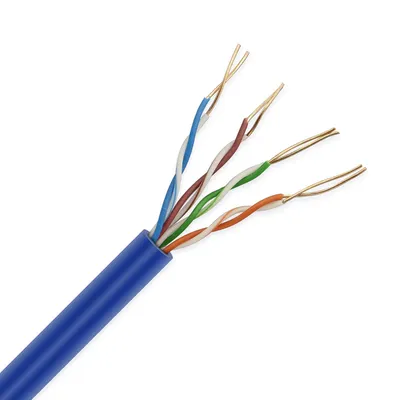
\includegraphics[width=0.6\textwidth]{images/Unshielded-Twisted-Pairs-Cable.jpg} % your file name
    \caption{Unshielded Twisted Pair Cables}
    \label{fig:network}
    \end{figure}
  \item \textbf{Shielded Twisted Pair Cables (STP):} These types of cables have extra insulation or protective covering over the conductors in the form of a copper braid covering. This covering provides strength to the overall structure of the cable. It also reduces noise and signal interference in the cable. The shielding ensures that the induced signal can be returned to the source via ground and only circulate around the shield without affecting the main propagating signal.
    \begin{figure}[h]
    \centering
    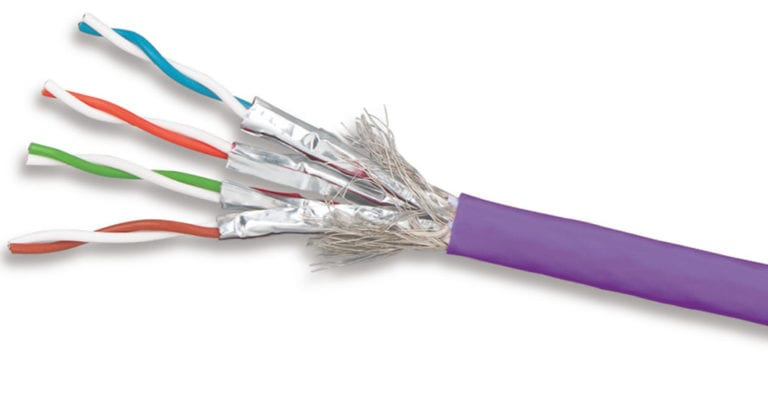
\includegraphics[width=0.6\textwidth]{images/Shielded-Twisted-Pairs-Cable.jpg} % your file name
    \caption{Shielded Twisted Pair Cables}
    \label{fig:network}
    \end{figure}
\end{itemize}
\subsubsection{Coaxial Cable:}
Coaxial Cable is a type of guided media made of Plastics, and copper wires which transmit the signal in electrical form rather than light form. Coaxial cable is also known as coax. The core copper conductor is used for the transmission of signals and the insulator is used to provide insulation to the copper conductor the insulator is surrounded by a braided metal conductor which helps to prevent the interference of electrical signals and prevent cross talk. This entire setup is again covered with a protective plastic layer to provide extra safety to the cable.
    \begin{figure}[h]
    \centering
    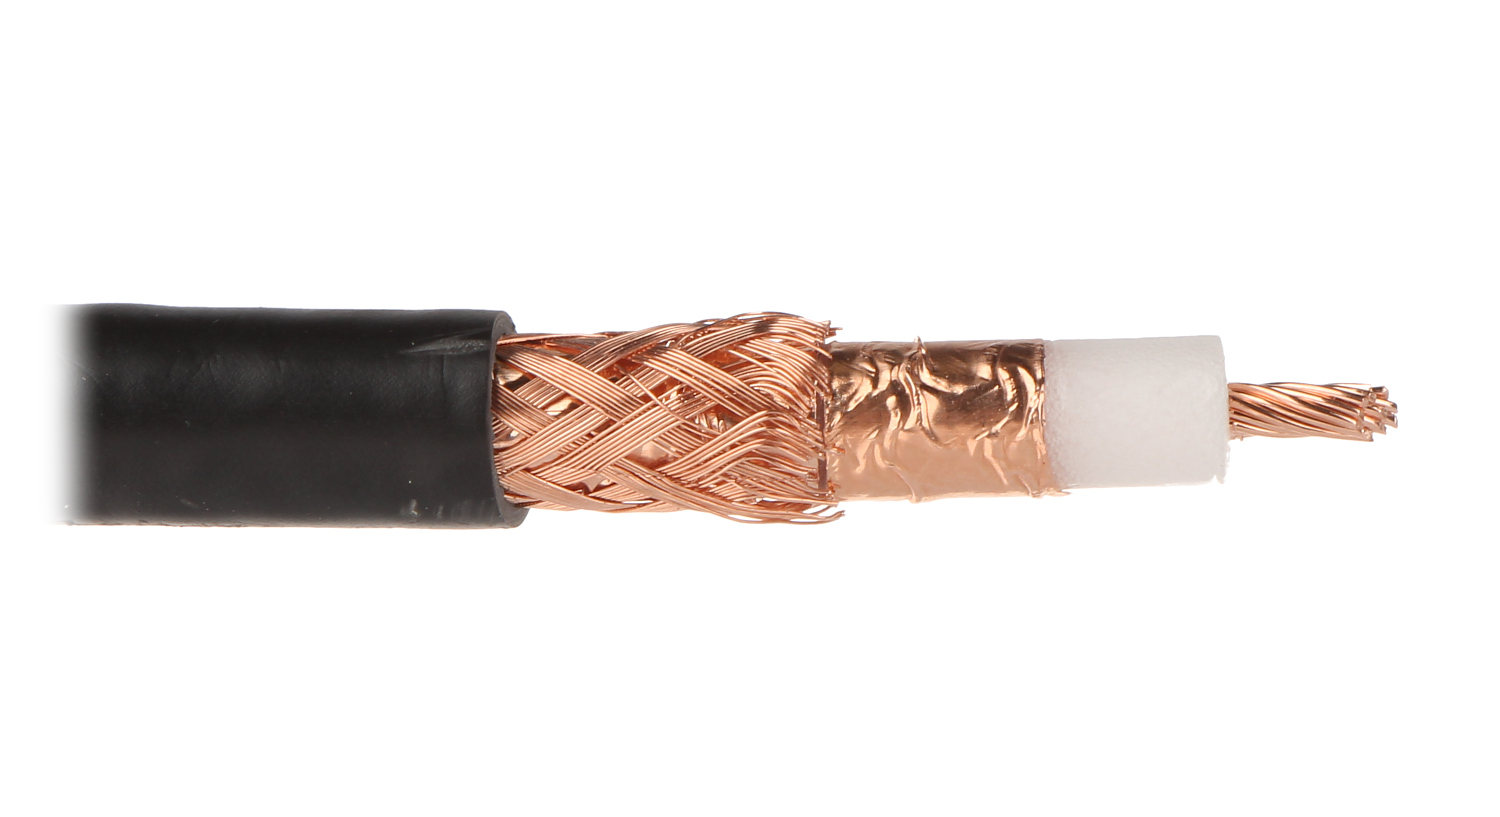
\includegraphics[width=0.6\textwidth]{images/Coaxial-Cable.jpg} % your file name
    \caption{Coaxial Cable}
    \label{fig:network}
    \end{figure}
\subsubsection{Fiber Optic Cable:}
Fiber-optic cabling is widely used for high-speed Ethernet links over relatively long distances. It uses glass or plastic fiber as a medium through which light is "guided" to the other end of the link. The fiber-optic cable itself has several layers made from different materials and having different functions. The most important layer is the core, which is the very center of the cable. A light source, called transmitter or Tx, shines a light into the core. The core itself is surrounded by optical material called the cladding that keeps the light in the core using an optical technique called total internal reflection. Together the cladding and core create the environment to allow transmission of light over the cable.
    \begin{figure}[H]
    \centering
    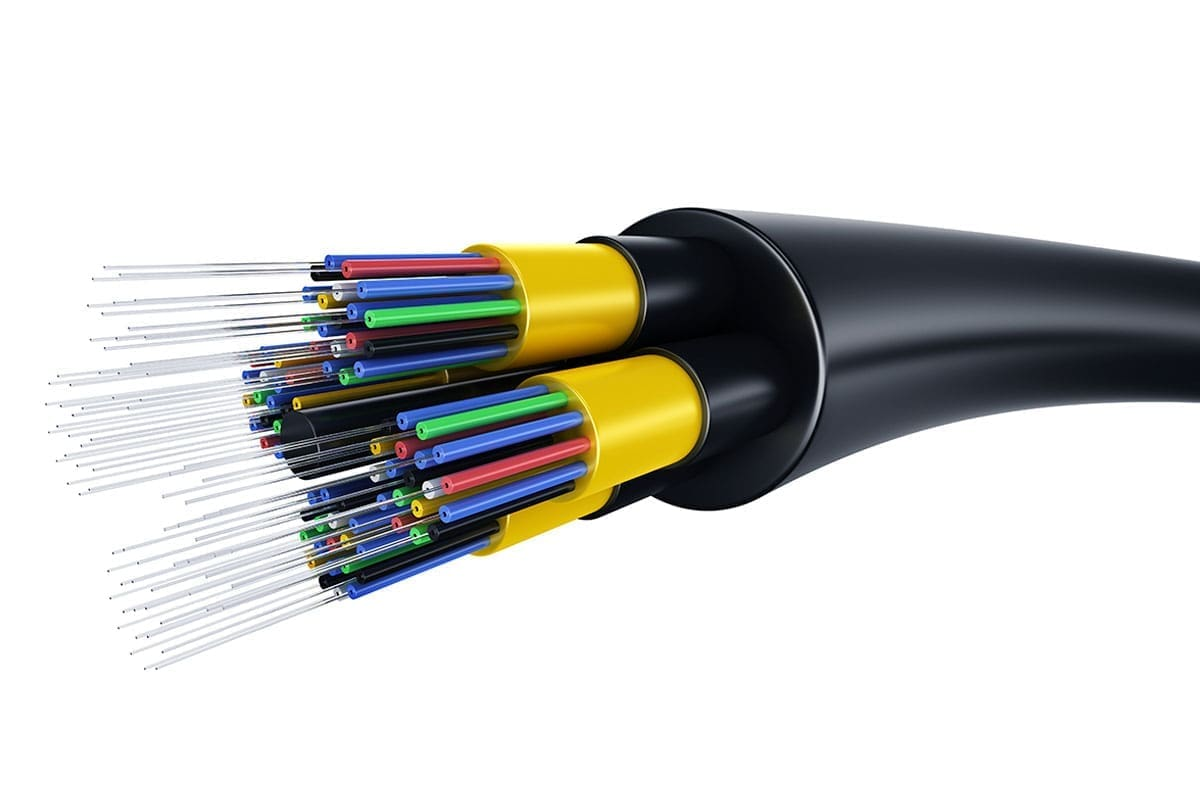
\includegraphics[width=0.6\textwidth]{images/optic-fiber-cable.jpg} % your file name
    \caption{Coaxial Cable}
    \label{fig:network}
    \end{figure}
\subsubsection{RJ45 Connector:}
An RJ45 (Registered Jack 45) is a standard connector used to terminate Ethernet cables like Cat5, Cat5e, and Cat6. It has 8 pins that connect to the 8 wires inside a twisted pair cable, enabling data transmission in LAN networks. RJ45 connectors are commonly used to connect computers, switches, and routers, and are essential for establishing wired network connections.
    \begin{figure}[H]
    \centering
    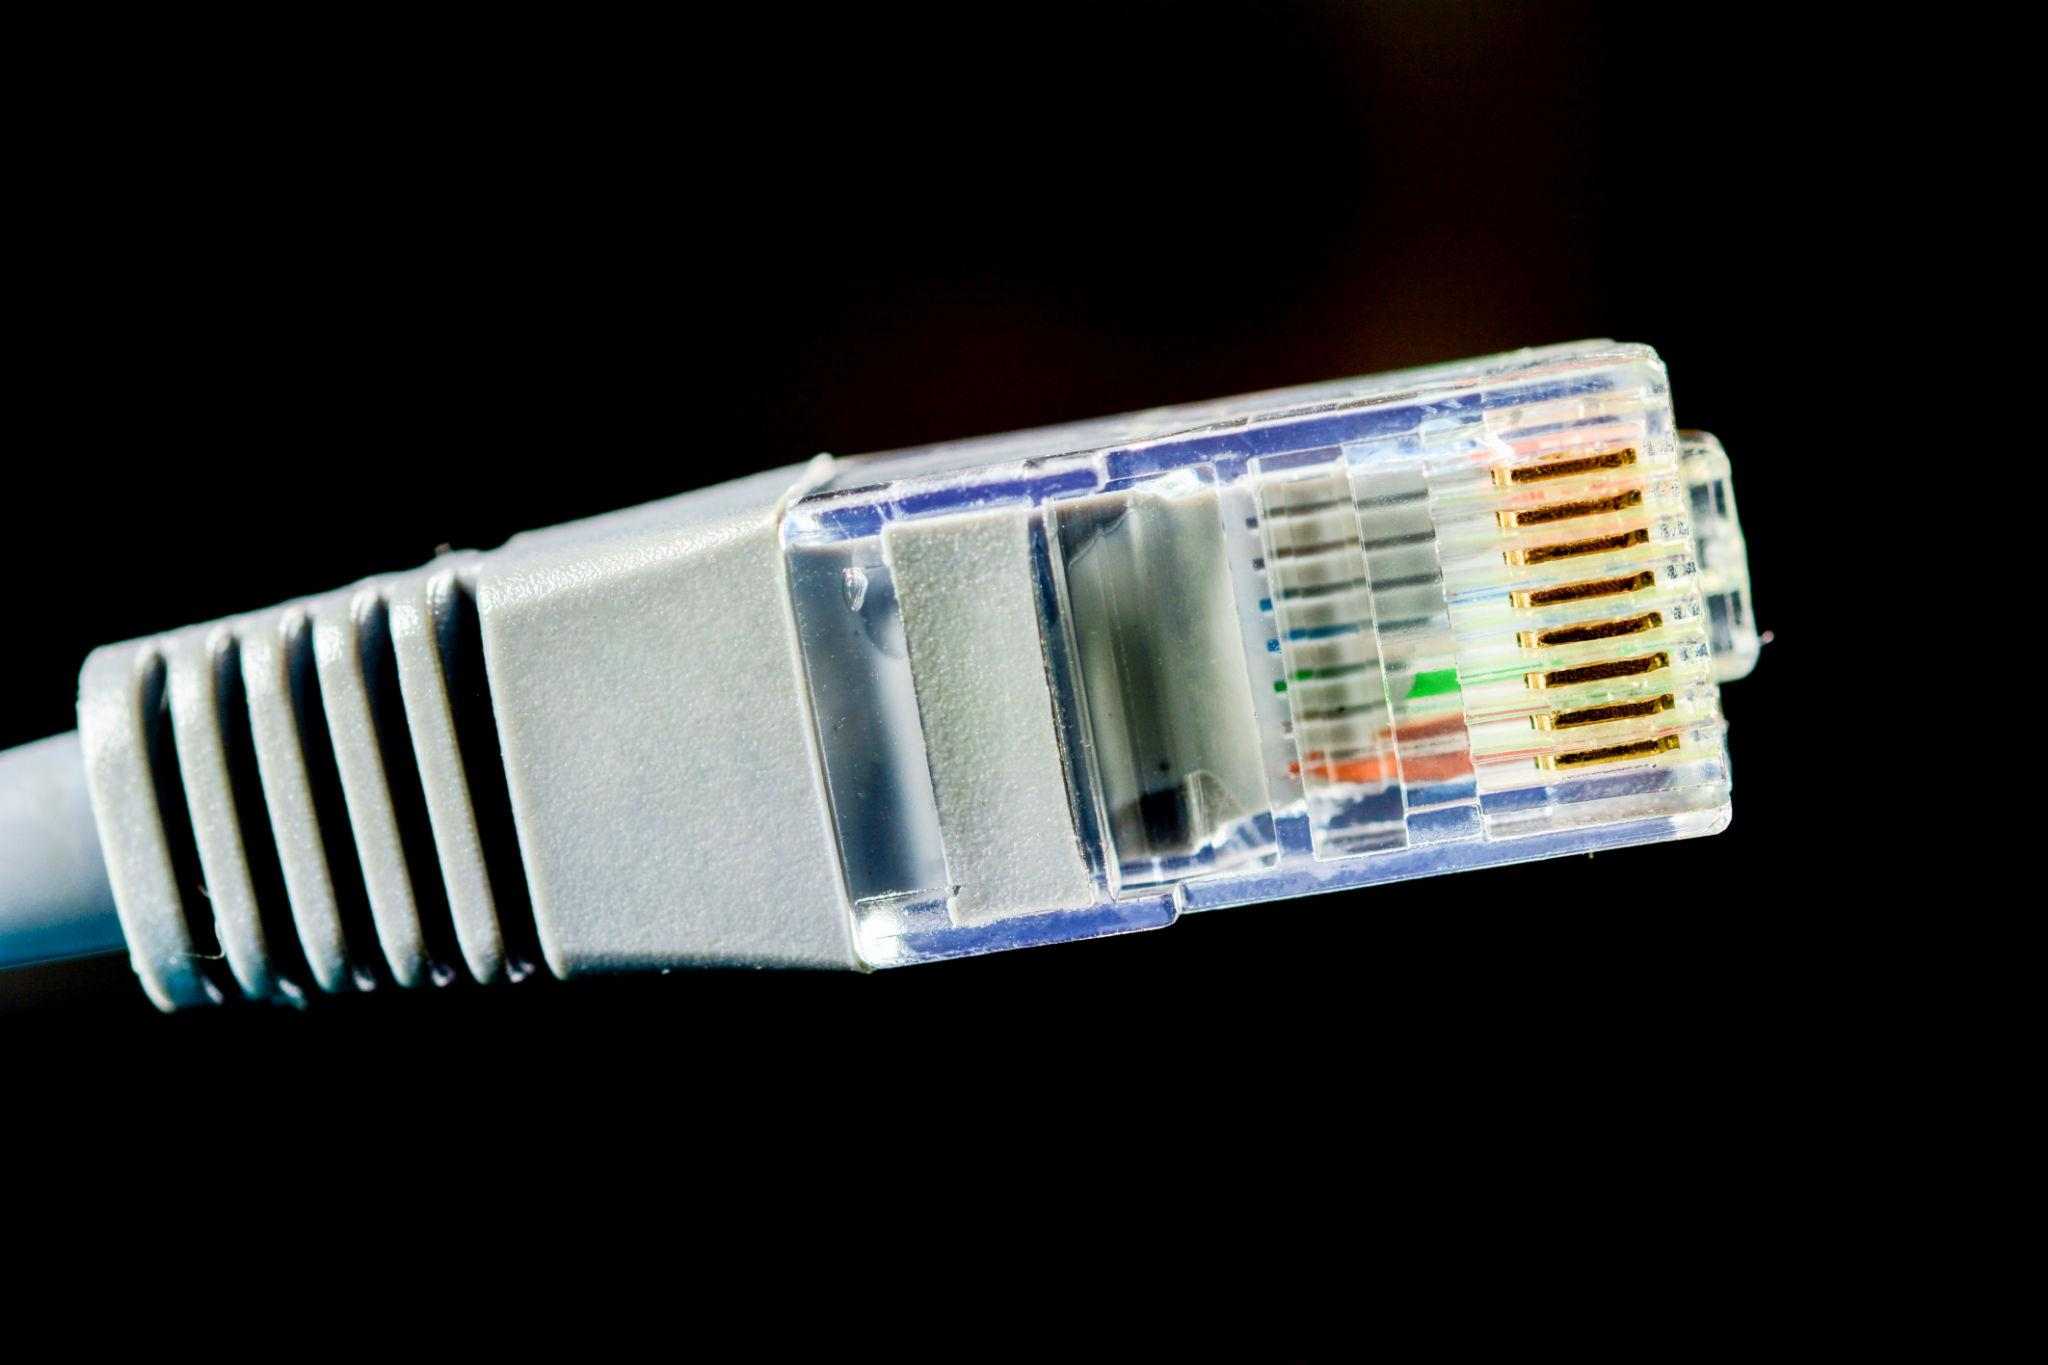
\includegraphics[width=0.6\textwidth]{images/RJ45-Connector.jpg} % your file name
    \caption{RJ45 Connector}
    \label{fig:network}
    \end{figure}
\subsubsection{BNC Connector:}
A BNC (Bayonet Neill–Concelman) connector is a type of coaxial cable connector that uses a bayonet locking mechanism for quick and secure connections. It is commonly used in CCTV systems, radio frequency applications, and older Ethernet networks. BNC connectors provide reliable signal transmission with good shielding, making them suitable for high-frequency signals and video connections.
    \begin{figure}[H]
    \centering
    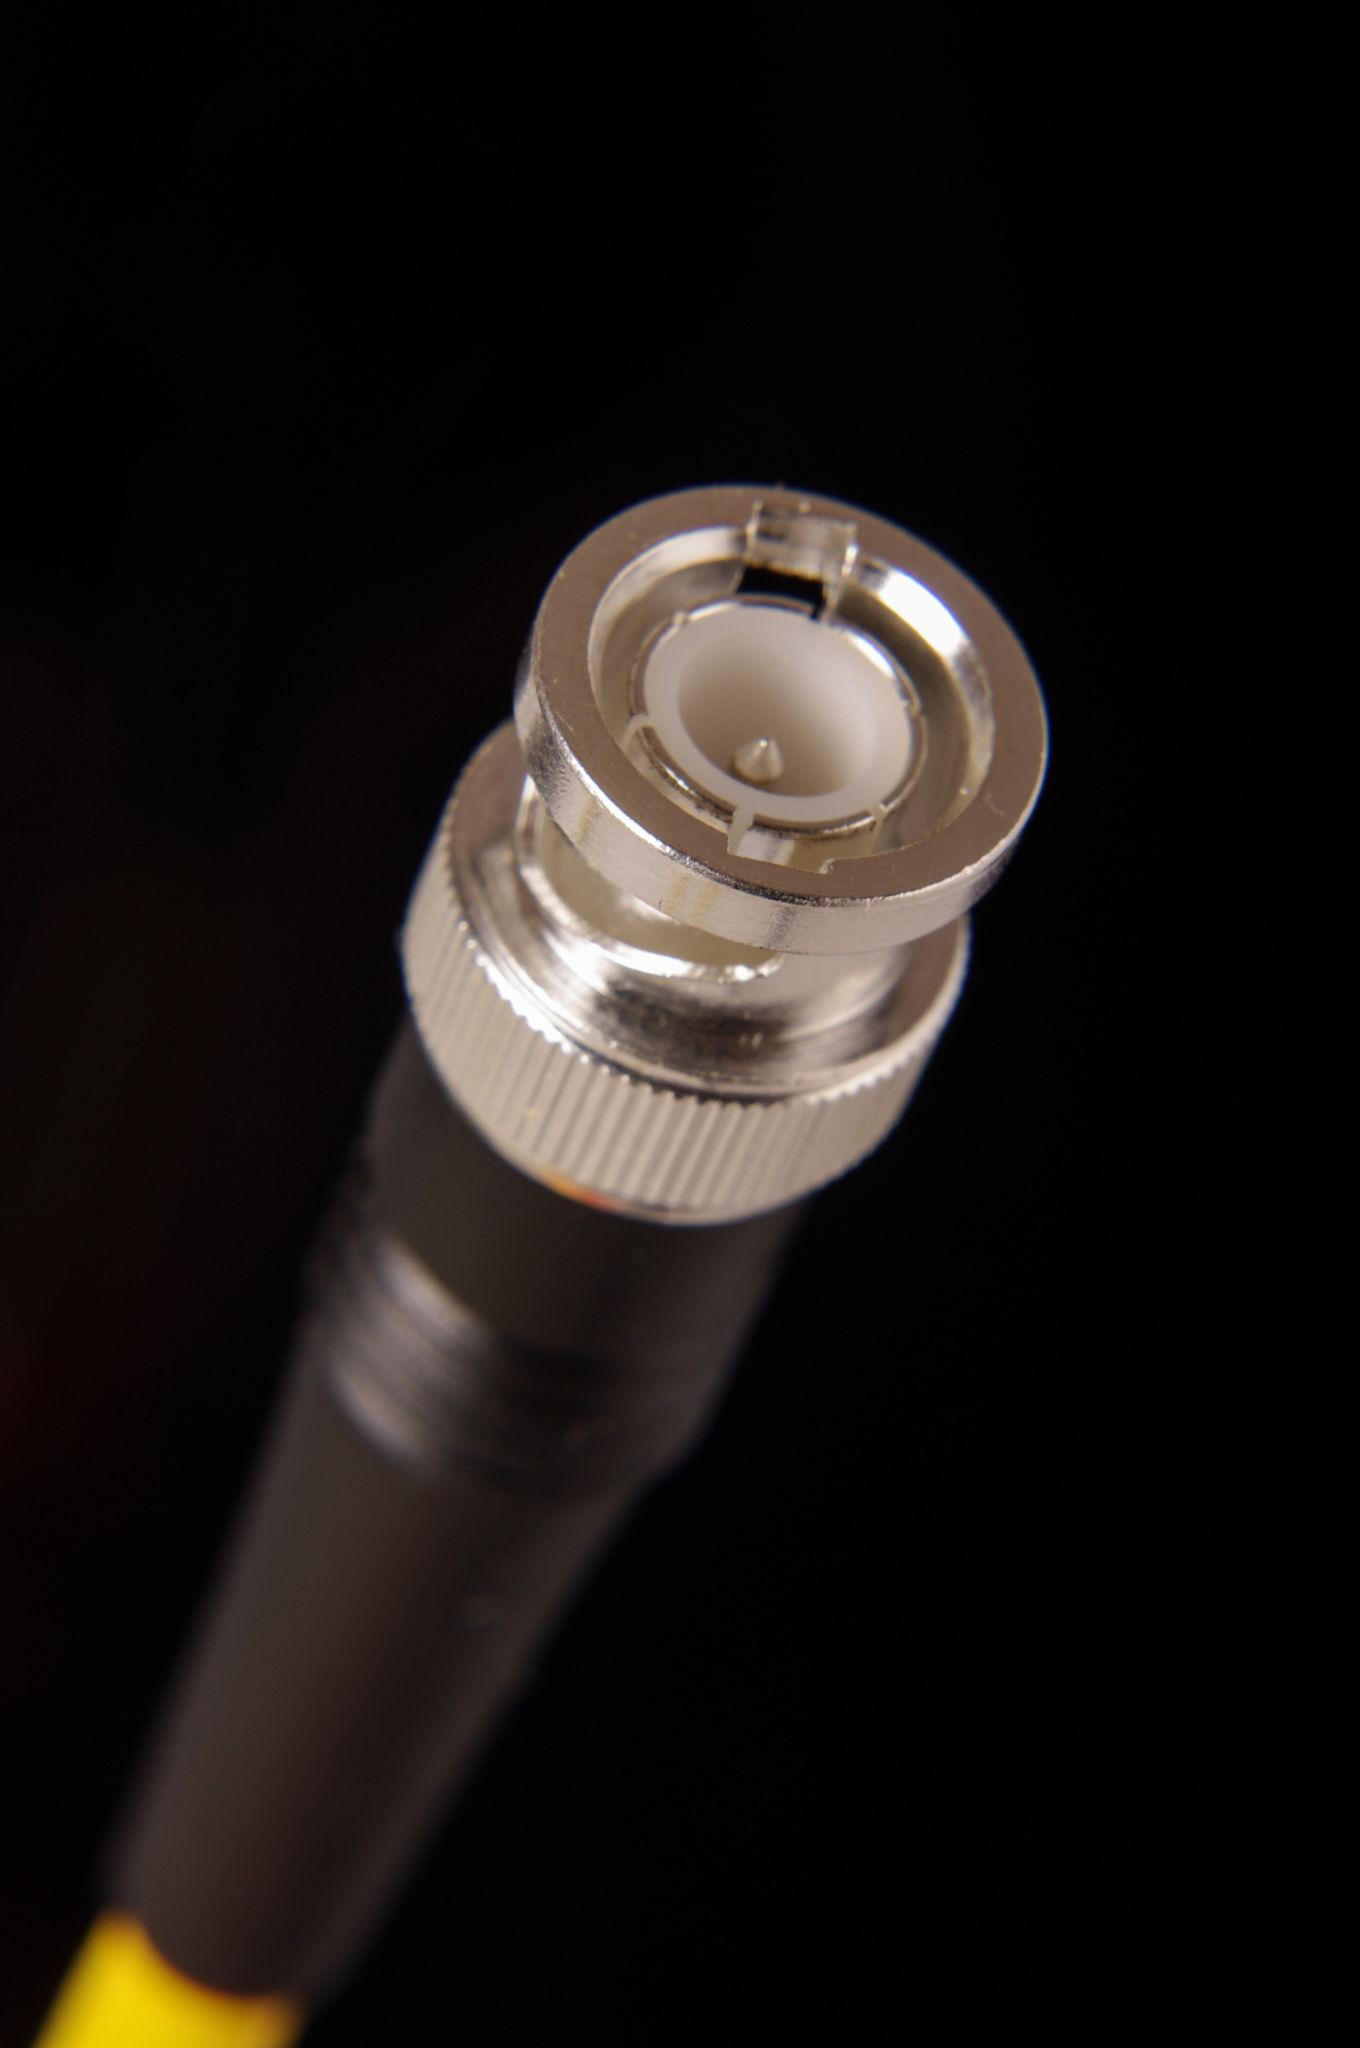
\includegraphics[width=0.6\textwidth]{images/BNC-Connector.jpg} % your file name
    \caption{BNC Connector}
    \label{fig:network}
    \end{figure}
    
\subsection{Apparatus/Equipments/Softwares:}
\begin{itemize}
    \item UTP Cable
    \item STP Cable
    \item Coaxial Cable
    \item Fiber Cable
    \item RJ45 Connectors
    \item BNC Connector
\end{itemize}

\subsection{Procedure:}
\begin{enumerate}
    \item Observe different cables physically
    \item Identify connectors used
    \item Note structure and purpose of each cable
\end{enumerate}

\subsection{Observation:}
Different types of cables and connectors were identified successfully.

\subsection{Viva Questions:}
\begin{enumerate}
    \item What is UTP cable?
    \item What is RJ45 connector?
    \item Which cable is fastest?
\end{enumerate}

% -------------------- EXPERIMENT - 02 --------------------
\newpage
\section{EXPERIMENT - 02}
\subsection{Title:}
Comparison of Cable Specifications

\subsection{Aim/Objective:}
To compare specifications of different networking cables.

\subsection{Theory:}
Different cables have different bandwidth, speed, and performance characteristics (e.g., Cat5 vs Cat6).
\begin{table}[h]
\centering
\begin{tabular}{lll}
\toprule
\textbf{Feature} & \textbf{Cat5 Cable} & \textbf{Cat6 Cable} \\
\midrule
Category           & Category 5           & Category 6                    \\
Bandwidth          & Up to 100 MHz        & Up to 250 MHz                 \\
Speed              & Up to 100 Mbps       & Up to 1 Gbps (10 Gbps short)  \\
Crosstalk          & More                 & Less                          \\
Internal Structure & Simple twisted pairs & Better insulation + separator \\
Cost               & Lower                & Higher                        \\
Usage              & Old networks         & Modern high-speed networks    \\
Performance        & Basic                & High                          \\
\bottomrule
\end{tabular}
\caption{Comparison between Cat5 and Cat6 Cables}
\end{table}

\subsection{Apparatus/Equipments/Softwares:}
\begin{itemize}
    \item Internet
    \item Datasheets
\end{itemize}

\subsection{Procedure:}
\begin{enumerate}
    \item Search specifications of Cat5, Cat6 cables
    \item Compare speed and bandwidth
    \item Prepare comparison table
\end{enumerate}

\subsection{Observation:}
Cat6 cable provides higher speed and bandwidth than Cat5.

\subsection{Viva Questions:}
\begin{enumerate}
    \item What is bandwidth?
    \item Difference between Cat5 and Cat6?
\end{enumerate}

% -------------------- EXPERIMENT - 03 --------------------
\newpage
\section{EXPERIMENT - 03}
\subsection{Title:}
Making Patch Cable (Crimping)

\subsection{Aim/Objective:}
To create a LAN cable using crimping tool.

\subsection{Theory:}
Crimping is the process of attaching connectors to cable ends using standards like T568A and T568B.

\subsection{Apparatus/Equipments/Softwares:}
\begin{itemize}
    \item UTP Cable
    \item RJ45 Connectors
    \item Crimping Tool
\end{itemize}

\subsection{Procedure:}
\subsubsection{Step 1: Strip the Outer Insulation}
\begin{itemize}
    \item Use a wire stripper or crimping tool
    \item Remove about 1–1.5 inches of the outer jacket
\end{itemize}
    \begin{figure}[h]
    \centering
    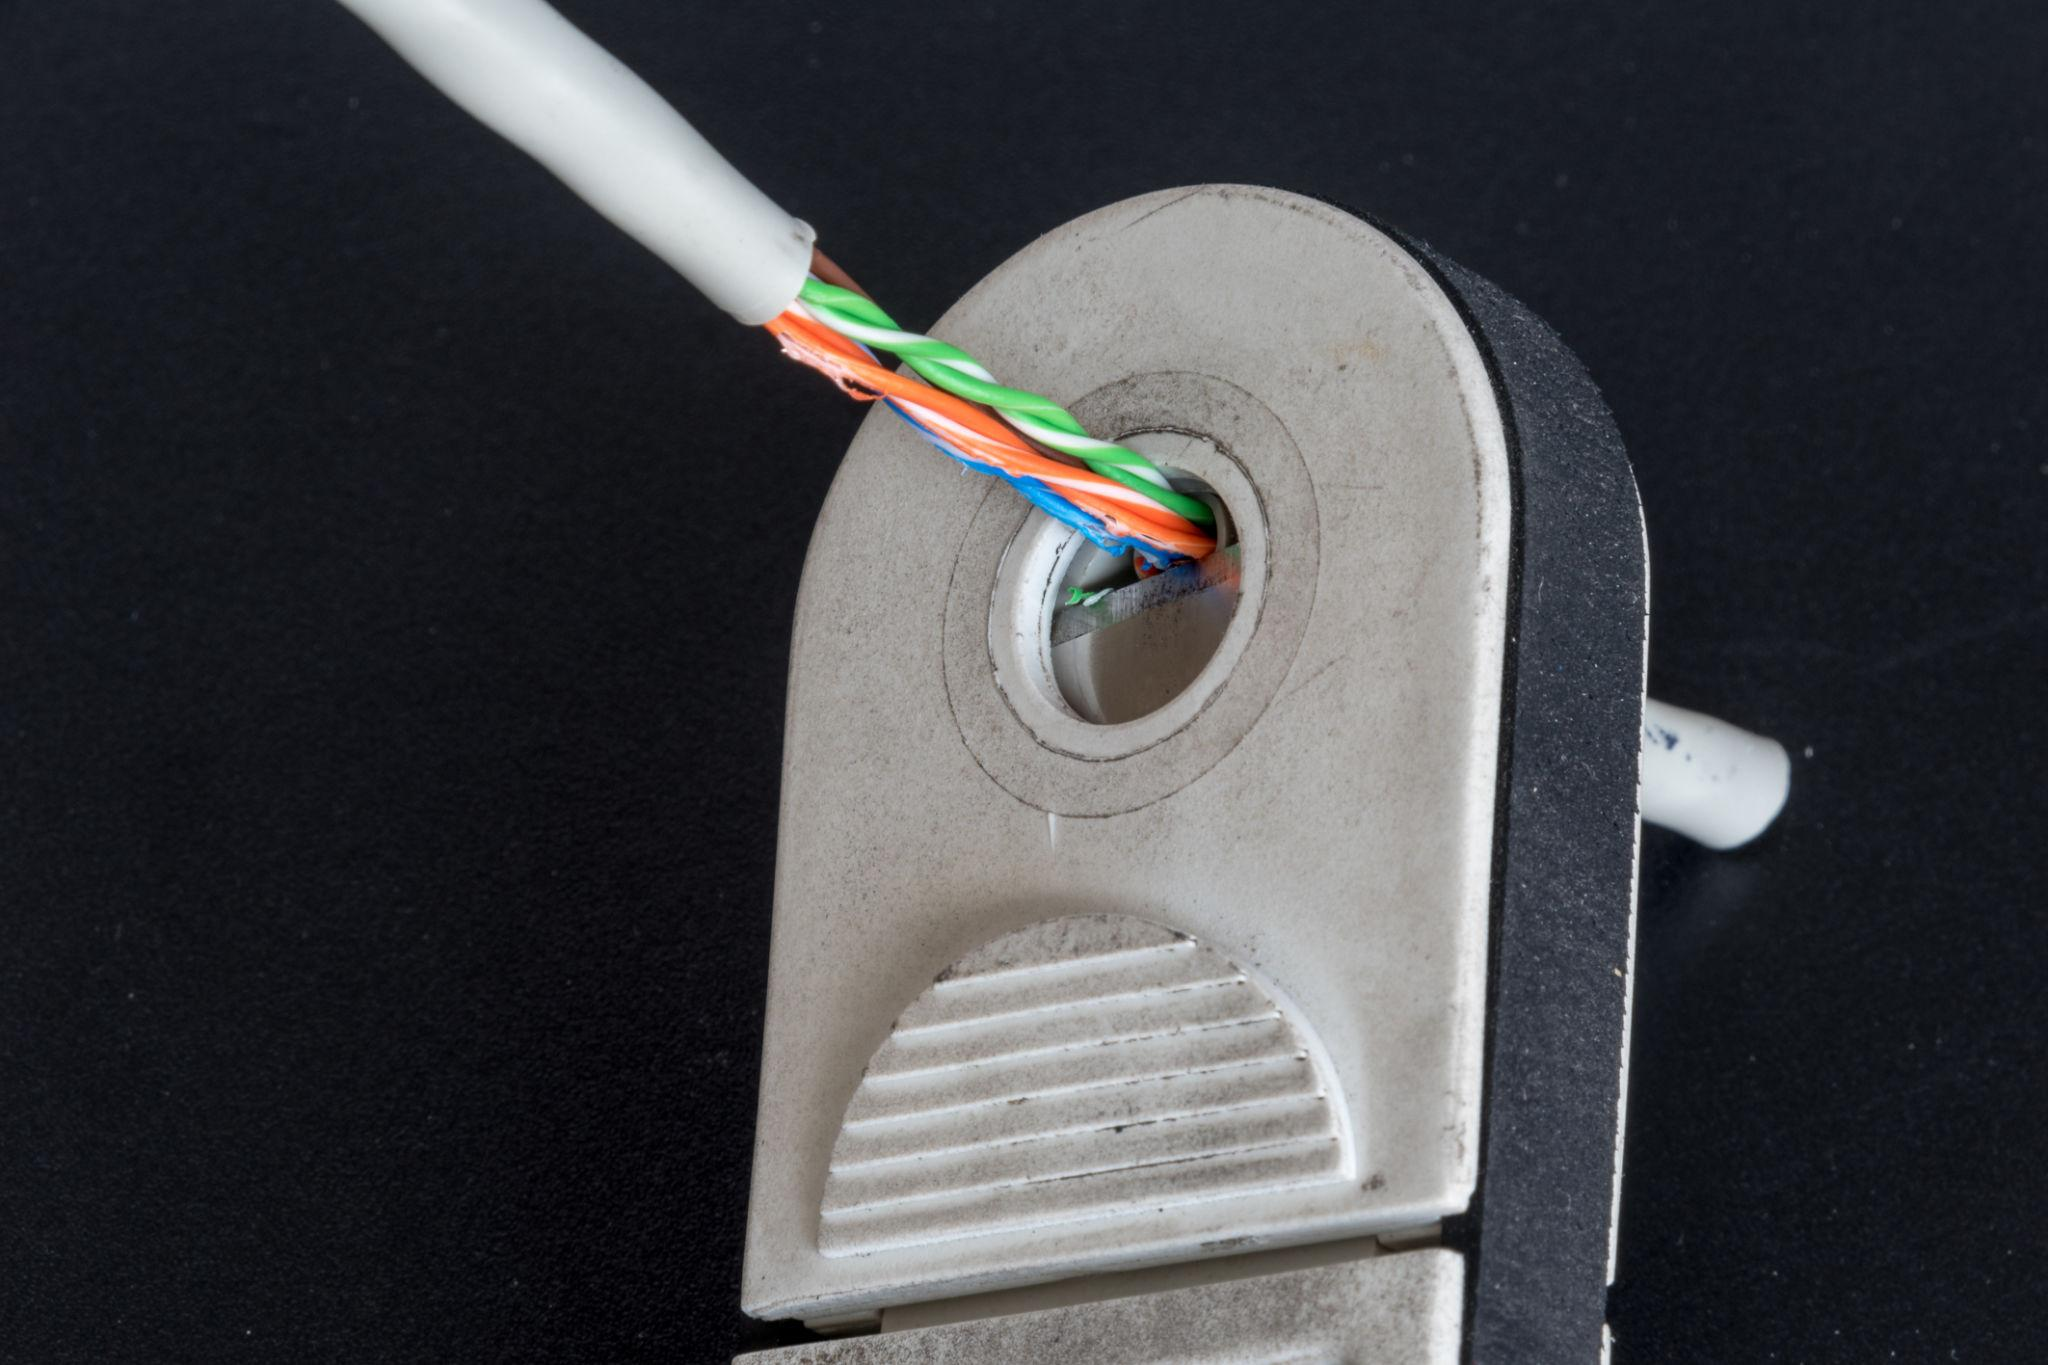
\includegraphics[width=0.6\textwidth]{images/3.1.jpg} 
    \caption{Strip the Outer Insulation}
    \label{fig:network}
    \end{figure}

\subsubsection{Step 2: Untwist and Arrange Wires (T568B Standard)}
\begin{itemize}
    \item Arrange wires in this exact T568B color order (left $\rightarrow$ right):
    \begin{enumerate}
        \item White-Orange
        \item Orange
        \item White-Green
        \item Blue
        \item White-Blue
        \item Green
        \item White-Brown
        \item Brown
    \end{enumerate}
    \item Straighten and align them neatly
\end{itemize}
    \begin{figure}[h]
    \centering
    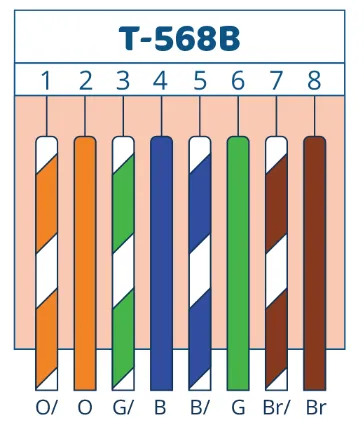
\includegraphics[width=0.6\textwidth]{images/3.2.jpg} 
    \caption{T568B color order}
    \label{fig:network}
    \end{figure}

\subsubsection{Step 3: Trim the Wires Evenly}
\begin{itemize}
    \item Cut wires to equal length (about 1–1.5 cm)
    \item Ensure all wires are perfectly aligned
\end{itemize}
    \begin{figure}[H]
    \centering
    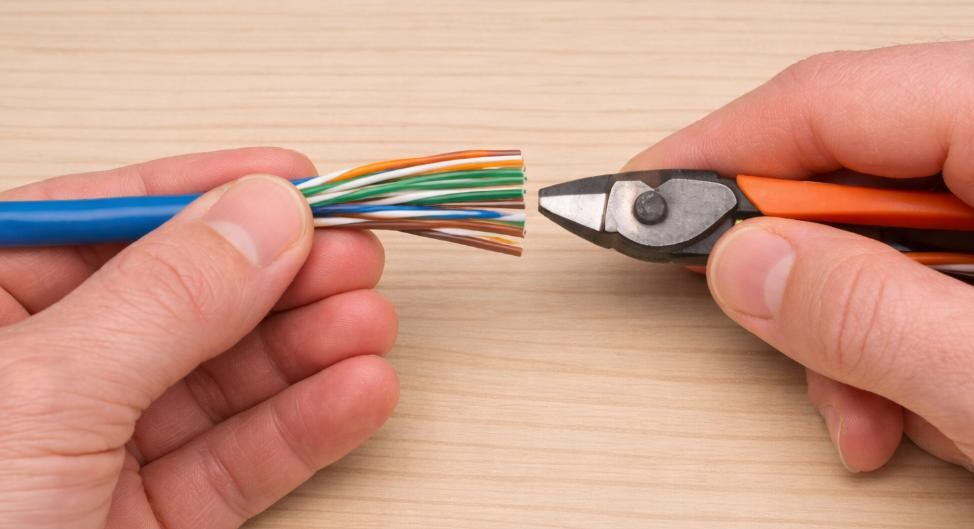
\includegraphics[width=0.6\textwidth]{images/3.3-1.jpg} 
    \caption{Trim the Wires Evenly}
    \label{fig:network}
    \end{figure}
    \begin{figure}[H]
    \centering
    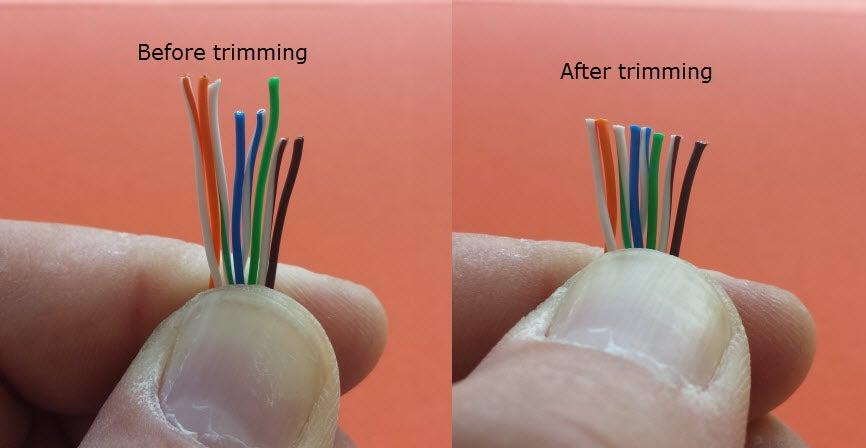
\includegraphics[width=0.6\textwidth]{images/3.3-2.jpg} 
    \caption{Before Trimming and After Trimming}
    \label{fig:network}
    \end{figure}

\subsubsection{Step 4: Insert Wires into RJ45 Connector}
\begin{itemize}
    \item Hold RJ45 clip facing downward
    \item Insert wires fully into connector
    \item Ensure each wire reaches the end and stays in order
\end{itemize}
    \begin{figure}[H]
    \centering
    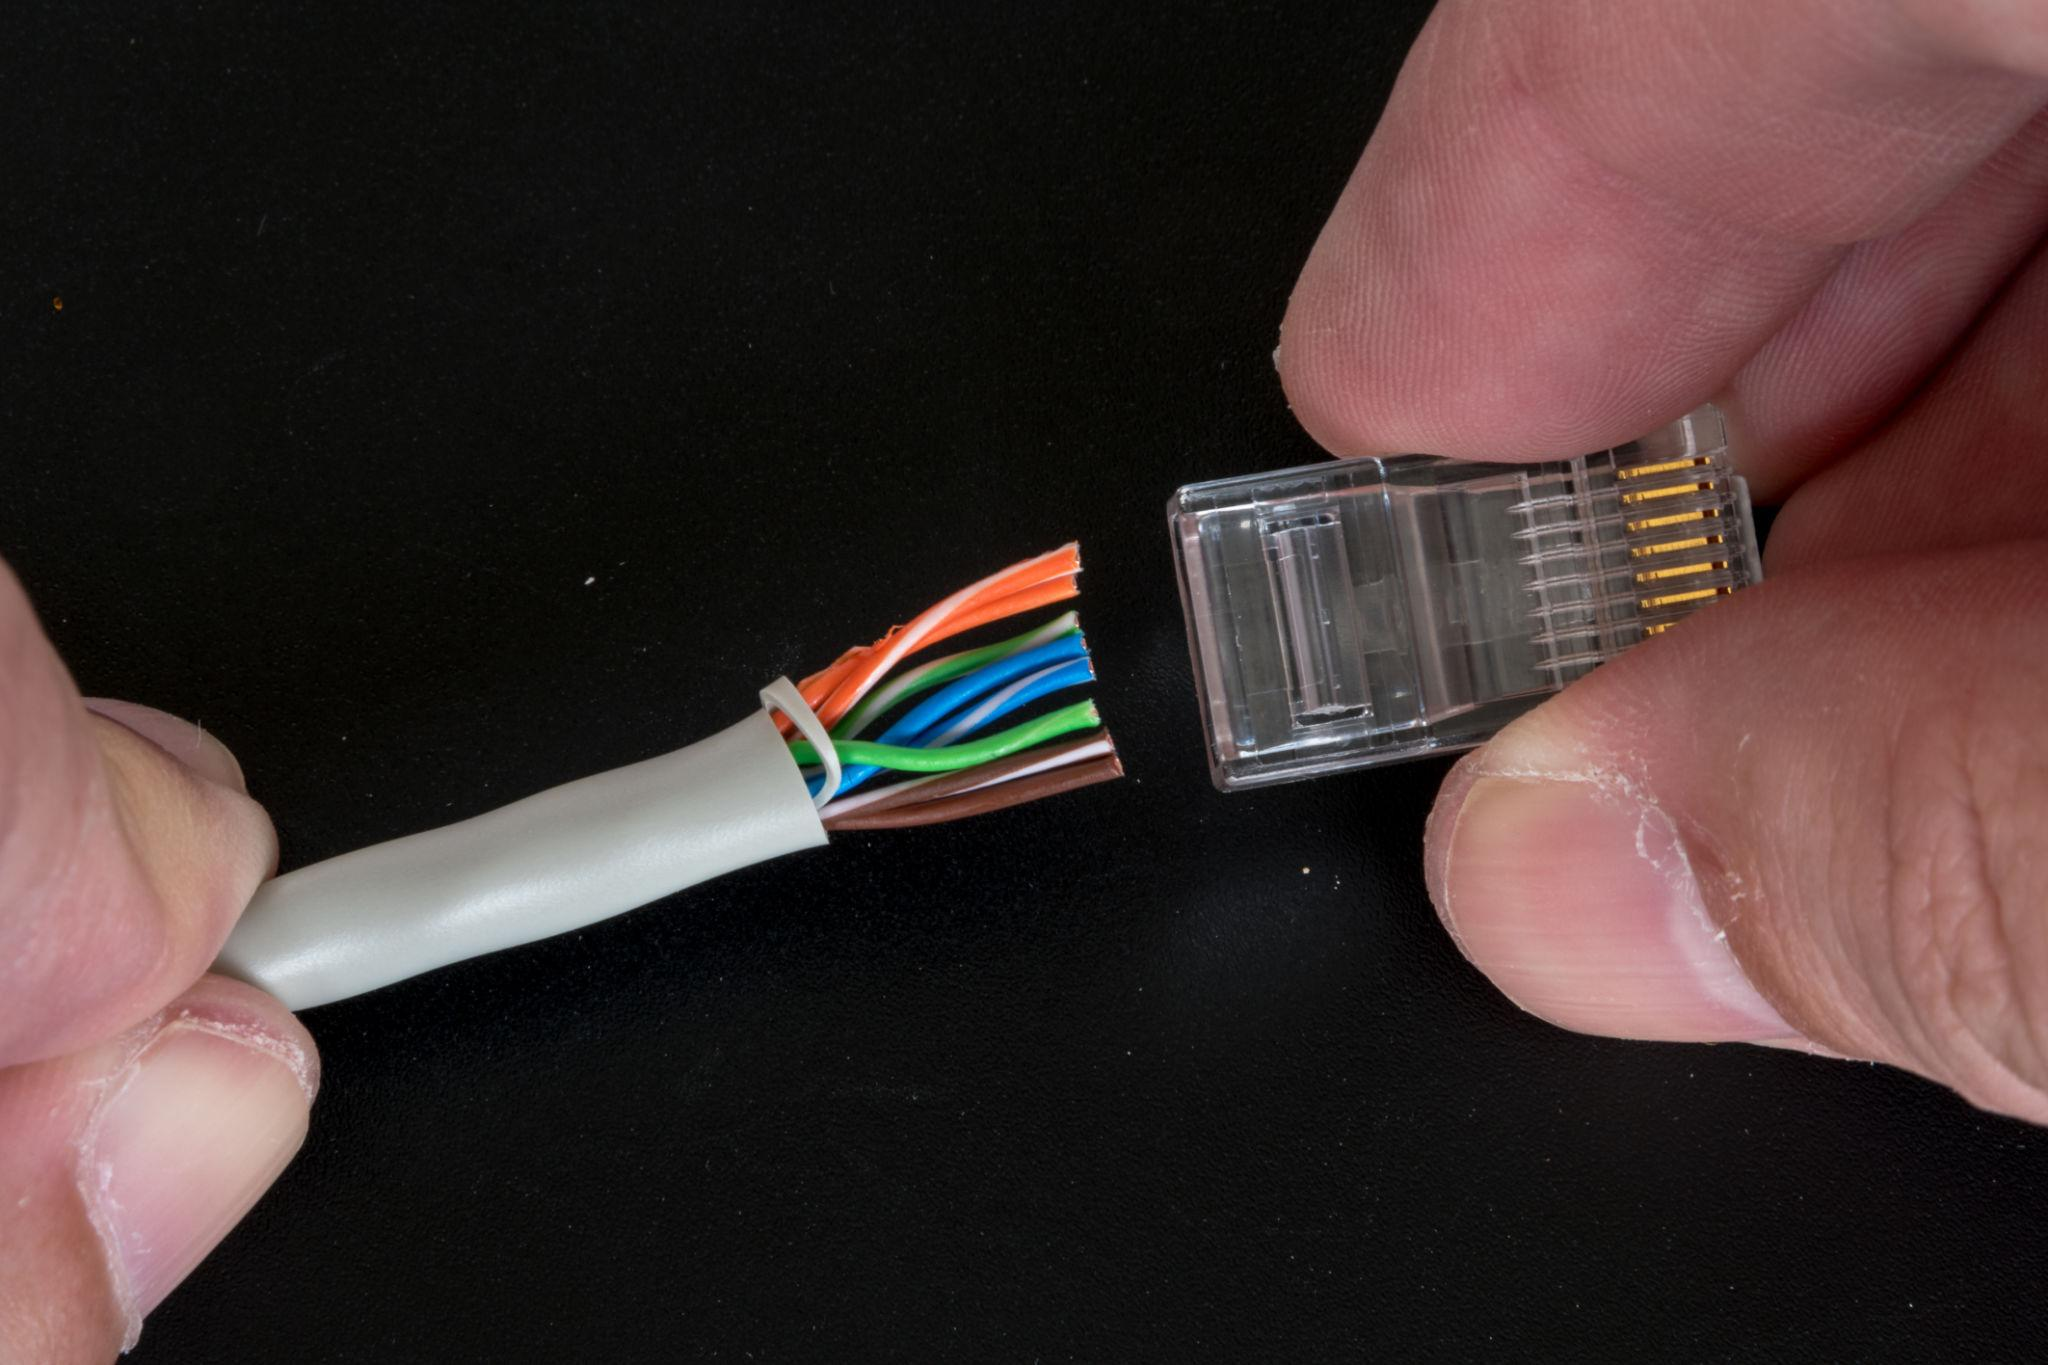
\includegraphics[width=0.6\textwidth]{images/3.4.jpg} 
    \caption{Insert Wires into RJ45 Connector}
    \label{fig:network}
    \end{figure}

\subsubsection{Step 5: Crimp the Connector}
\begin{itemize}
    \item Place connector into crimping tool
    \item Press firmly until it clicks
    \item Pins will pierce wires to make contact
\end{itemize}
    \begin{figure}[H]
    \centering
    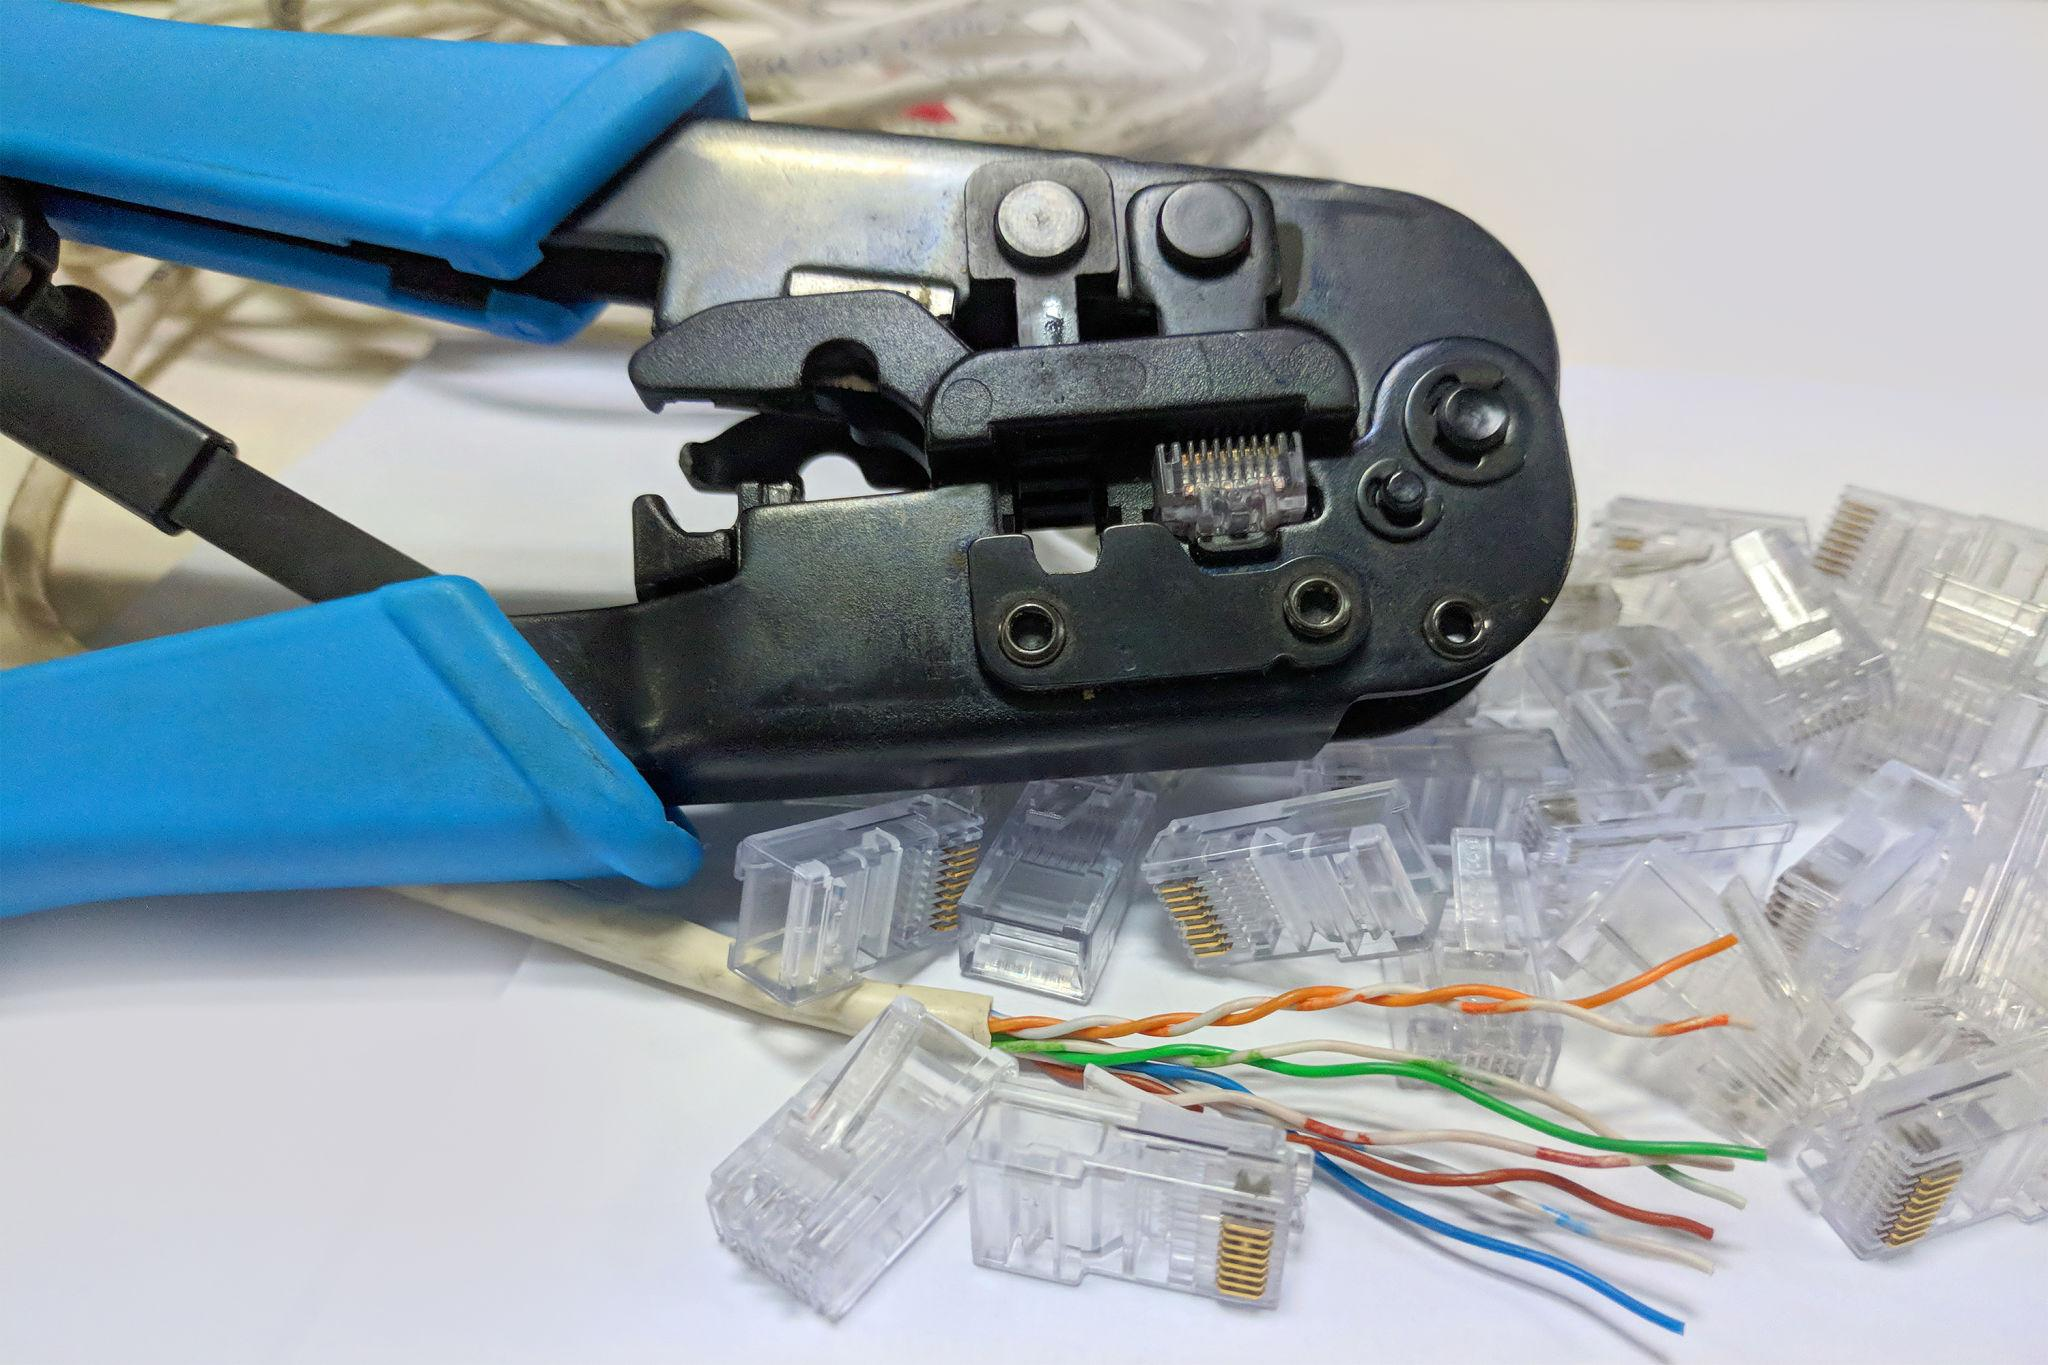
\includegraphics[width=0.6\textwidth]{images/3.5.jpg} 
    \label{fig:network}
    \end{figure}

\subsection{Observation:}
Patch cable was successfully created.

\subsection{Viva Questions:}
\begin{itemize}
    \item What is crimping?
    \item What is T568B standard?
\end{itemize}

% -------------------- EXPERIMENT - 04 --------------------
\newpage
\section{EXPERIMENT - 04}
\subsection{Title:}
Testing of Network Cable

\subsection{Aim/Objective:}
To test LAN cable using cable tester.

\subsection{Theory:}
Cable testers check continuity, faults, and correct wiring of cables.

\subsection{Apparatus/Equipments/Softwares:}
\begin{itemize}
    \item Cable Tester
\end{itemize}

\subsection{Procedure:}
\subsubsection{Step 1: Connect Cable to Tester}
\begin{itemize}
    \item Plug one end of the cable into the main unit
    \item Plug the other end into the remote unit
    \item Ensure both ends are securely connected
\end{itemize}
    \begin{figure}[H]
    \centering
    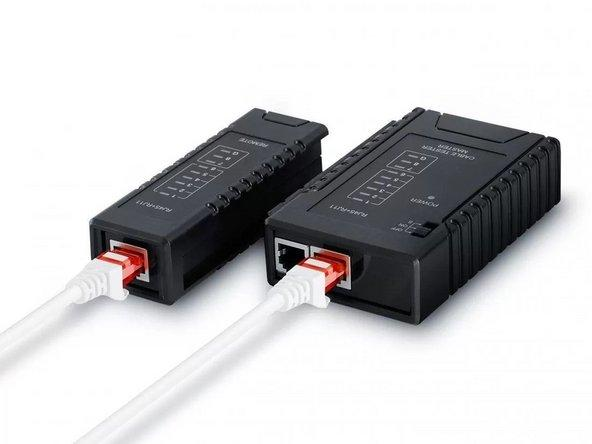
\includegraphics[width=1\textwidth]{images/4.1.jpg} 
    \label{fig:network}
    \end{figure}

\subsubsection{Step 2: Turn On the Tester}
\begin{itemize}
    \item Switch ON the tester
    \item Some testers have modes: Auto / Manual / Slow
    \item Choose Auto mode for continuous testing
\end{itemize}
    \begin{figure}[H]
    \centering
    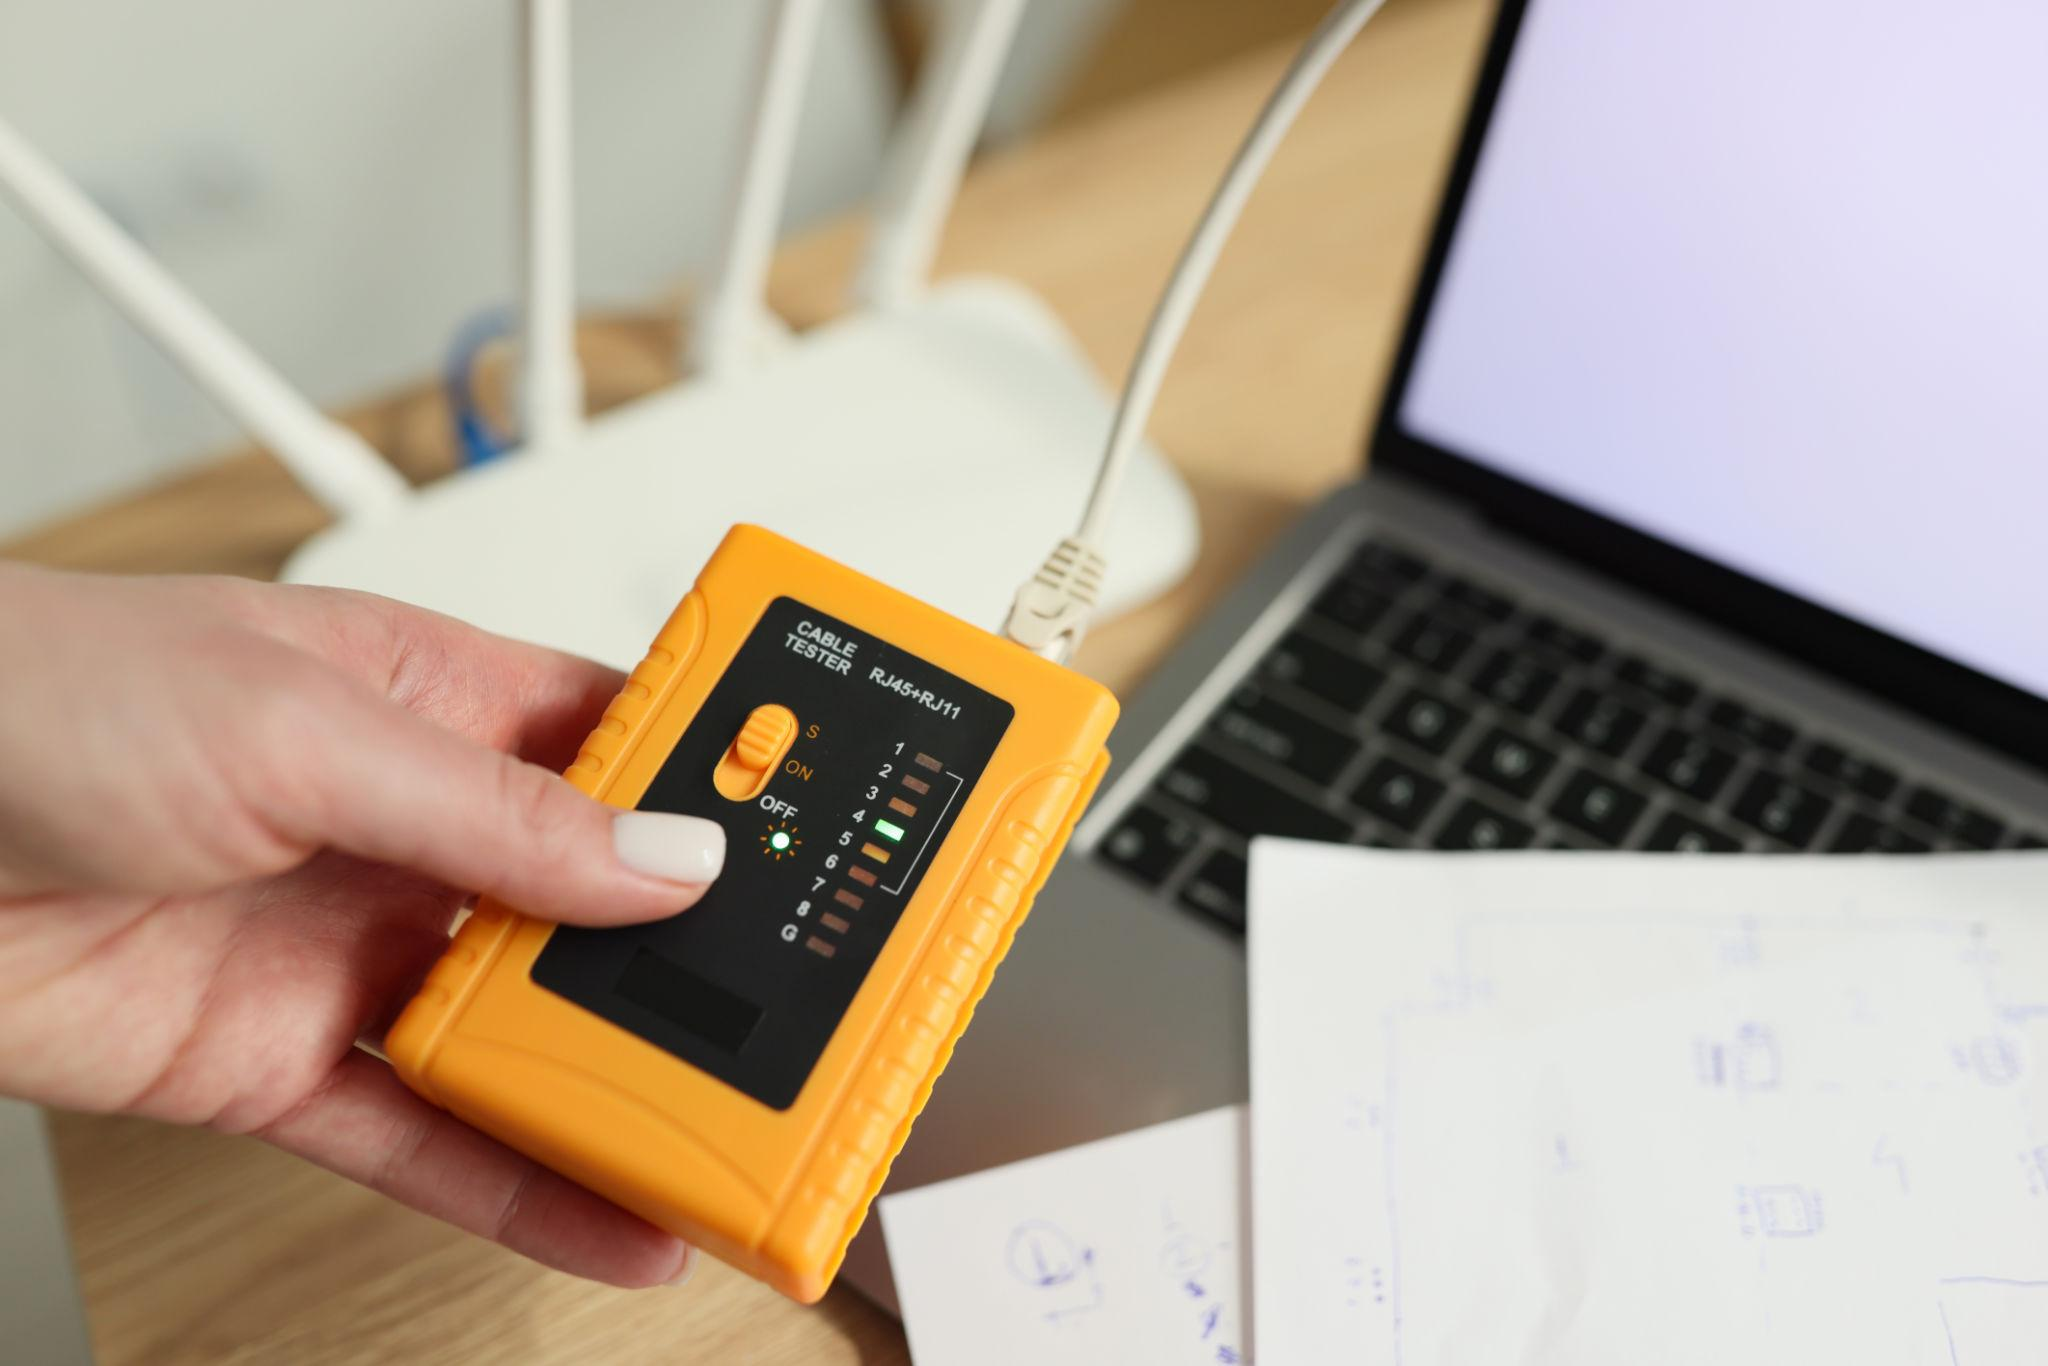
\includegraphics[width=1\textwidth]{images/4.2.jpg} 
    \label{fig:network}
    \end{figure}

\subsubsection{Step 3: Observe LED Sequence}
\begin{itemize}
    \item LEDs will glow in sequence: 1 \rightarrow 2 \rightarrow 3 \rightarrow 4 \rightarrow 5 \rightarrow 6 \rightarrow 7 \rightarrow 8
    \item Both main and remote unit should show the same order
\end{itemize}

\subsubsection{Step 4: Identify Faults (if any)}
Common faults:
\begin{itemize}
    \item Open circuit \rightarrow LED does not glow
    \item Short circuit \rightarrow Multiple LEDs glow together
    \item Crossed wires \rightarrow Wrong sequence (e.g., 1\rightarrow3\rightarrow2)
    \item Miswiring \rightarrow LEDs mismatch between main \& remote
\end{itemize}

\subsubsection{Step 5: Confirm Cable Status}
\begin{itemize}
    \item All LEDs in correct order \rightarrow Cable is GOOD
    \item Any mismatch \rightarrow Cable is FAULTY
\end{itemize}

\subsection{Observation:}
Cable showed proper continuity and working condition.

\subsection{Viva Questions:}
\begin{enumerate}
    \item What is continuity?
    \item What is cable fault?
\end{enumerate}

% -------------------- EXPERIMENT - 05 --------------------
\newpage
\section{EXPERIMENT - 05}
\subsection{Title:}
IP Address Configuration

\subsection{Aim/Objective:}
To configure IP address, gateway and DNS.

\subsection{Theory:}
IP address uniquely identifies a device in a network. Gateway connects networks and DNS resolves domain names.

\subsection{Apparatus/Equipments/Softwares:}
\begin{itemize}
    \item PC / Laptop
\end{itemize}

\subsection{Procedure:}
\subsubsection{Step 1: Open Network Settings}
\begin{itemize}
    \item Go to \texttt{Control Panel} \rightarrow \texttt{Network and Internet} \rightarrow \texttt{Network and Sharing Center}
    \item Click \texttt{Change adapter settings}
    \item Right-click \texttt{Ethernet / Wi-Fi} \rightarrow \texttt{Properties}
\end{itemize}
    \begin{figure}[H]
    \centering
    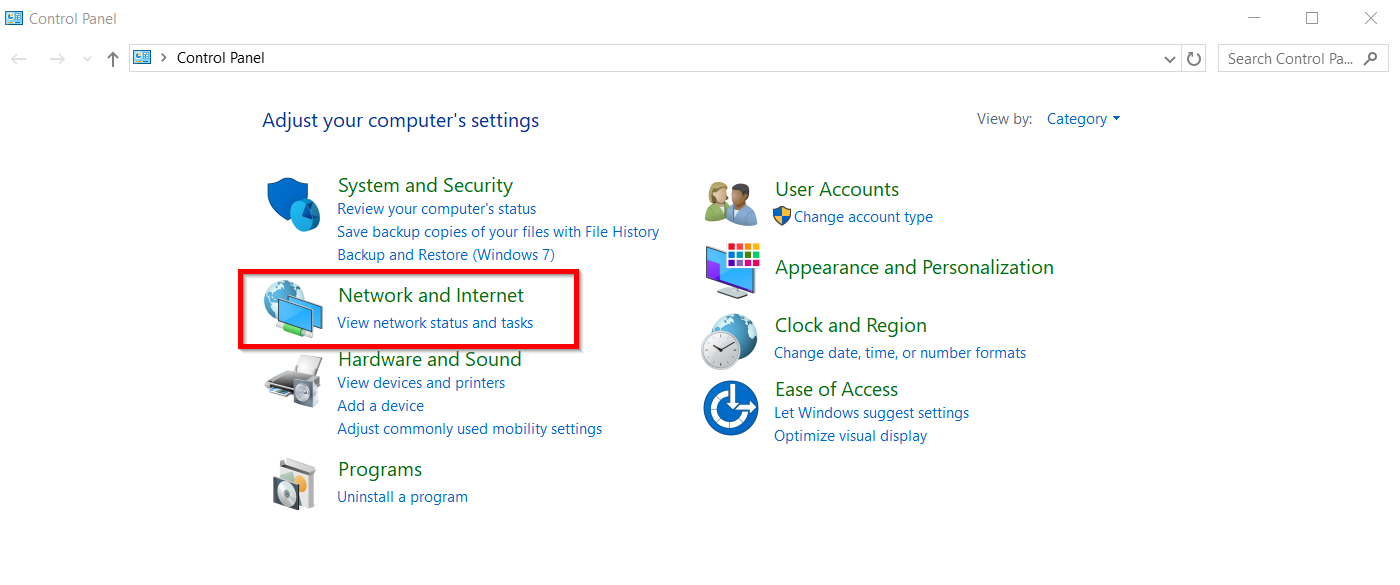
\includegraphics[width=1\textwidth]{images/5.1-1.png} 
    \label{fig:network}
    \end{figure}
    \begin{figure}[H]
    \centering
    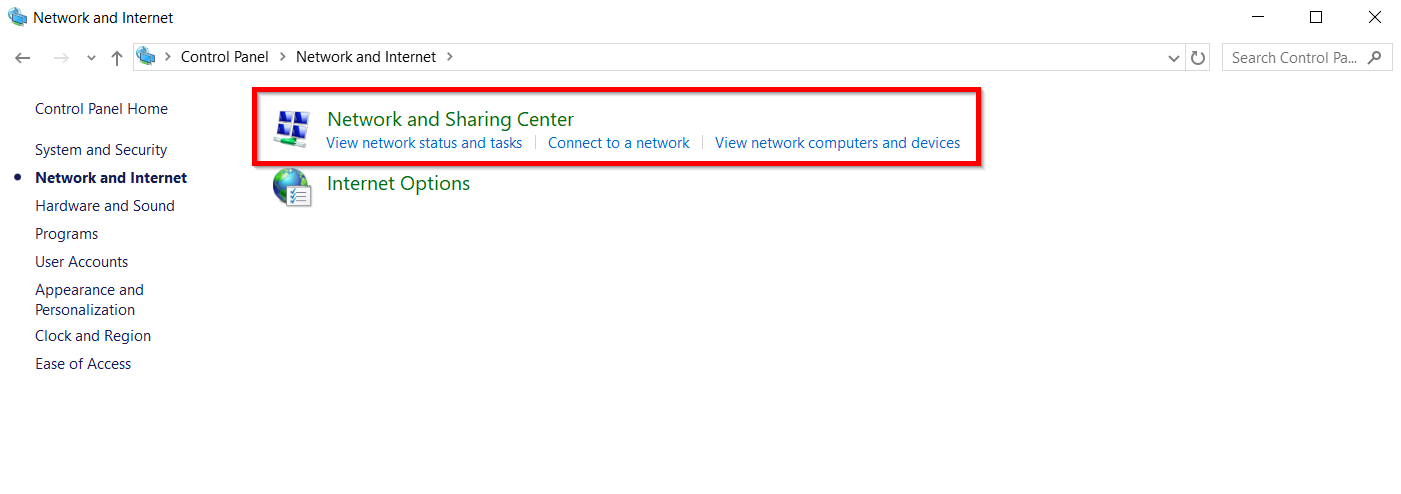
\includegraphics[width=1\textwidth]{images/5.1-2.png} 
    \label{fig:network}
    \end{figure}
    \begin{figure}[H]
    \centering
    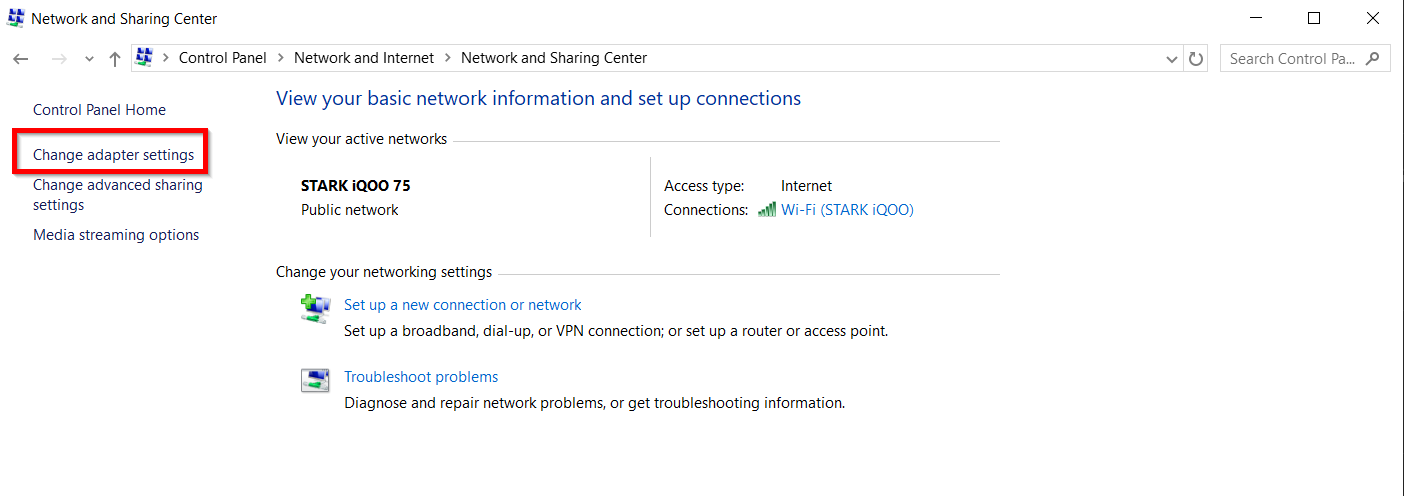
\includegraphics[width=1\textwidth]{images/5.1-3.png} 
    \label{fig:network}
    \end{figure}
    \begin{figure}[H]
    \centering
    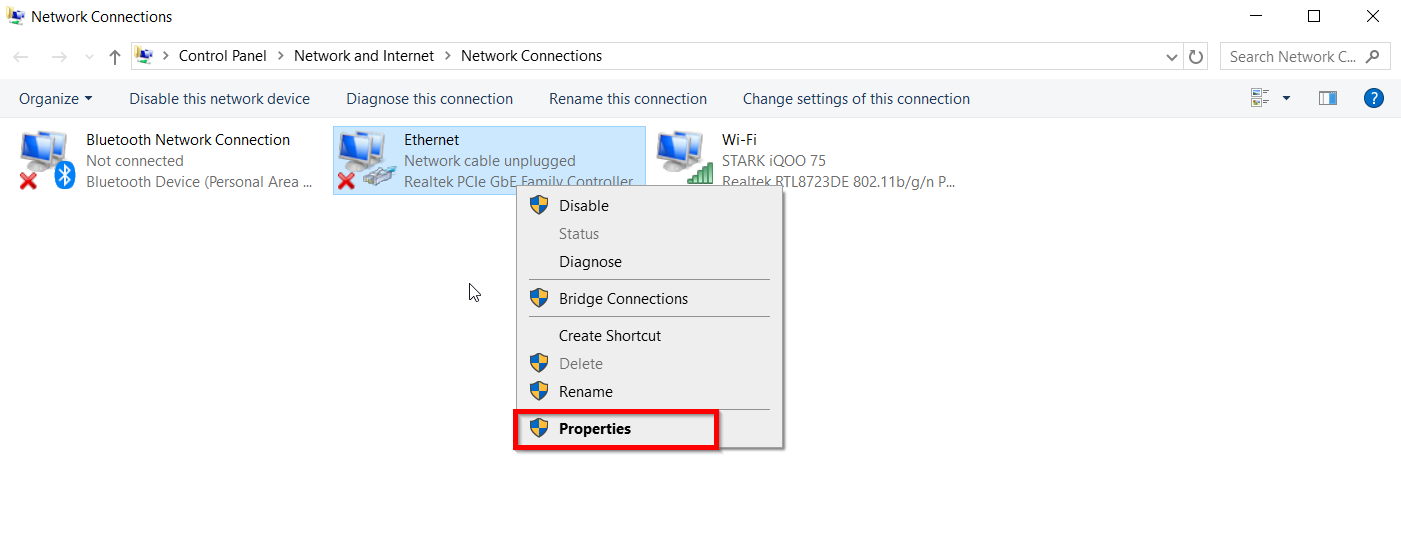
\includegraphics[width=1\textwidth]{images/5.1-4.png} 
    \label{fig:network}
    \end{figure}

\subsubsection{Step 2: Select IPv4 Settings}
\begin{itemize}
    \item Select \texttt{Internet Protocol Version 4 (TCP / IPv4)}
    \item Click \texttt{Properties}
\end{itemize}
    \begin{figure}[H]
    \centering
    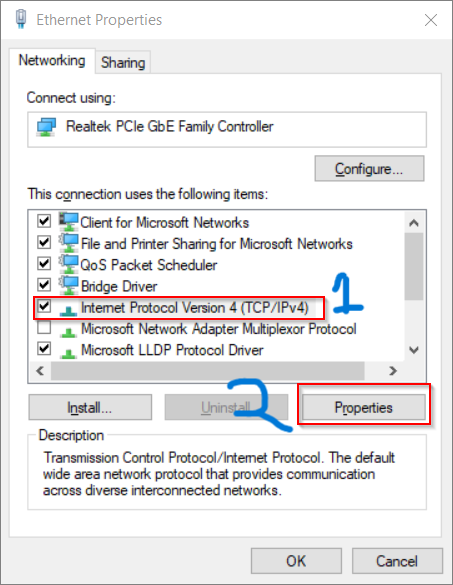
\includegraphics[width=1\textwidth]{images/5.2.png} 
    \label{fig:network}
    \end{figure}

\subsubsection{Step 3: Set IP Address Manually}
Choose “\texttt{Use the following IP address}” and enter:
\begin{itemize}
    \item IP Address: \texttt{10.133.133.150}
    \item Subnet Mask: \texttt{255.255.255.0}
    \item Default Gateway: \texttt{10.133.133.191}
\end{itemize}
These values depend on your network
    \begin{figure}[H]
    \centering
    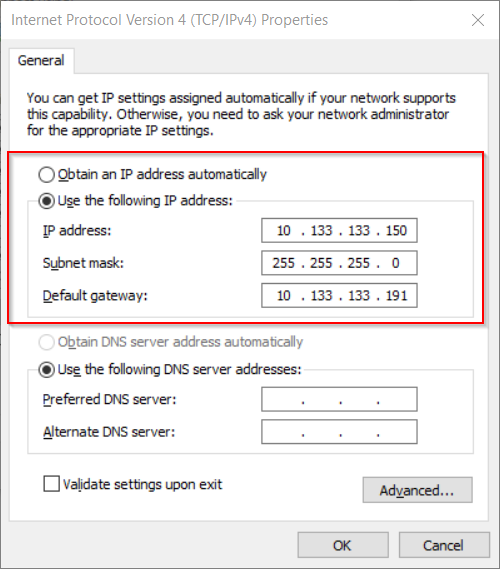
\includegraphics[width=1\textwidth]{images/5.3.png} 
    \label{fig:network}
    \end{figure}

\subsubsection{Step 4: Configure DNS Server}
Choose “\texttt{Use the following DNS server addresses}” and enter:
\begin{itemize}
    \item Preferred DNS: \texttt{8.8.8.8}
    \item Alternate DNS: \texttt{8.8.4.4}
\end{itemize}
These are public DNS servers (Google DNS)
    \begin{figure}[H]
    \centering
    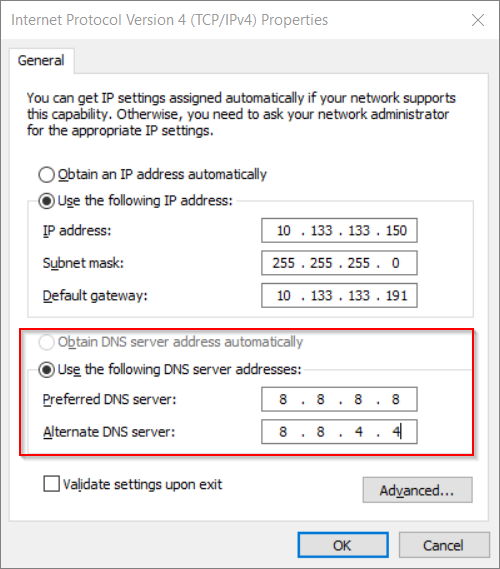
\includegraphics[width=1\textwidth]{images/5.4.png} 
    \label{fig:network}
    \end{figure}

\subsubsection{Step 5: Save Settings}
Choose “\texttt{Use the following DNS server addresses}” and enter:
\begin{itemize}
    \item Click \texttt{OK} \rightarrow \texttt{Close}
    \item Your IP configuration is now applied
\end{itemize}
    \begin{figure}[H]
    \centering
    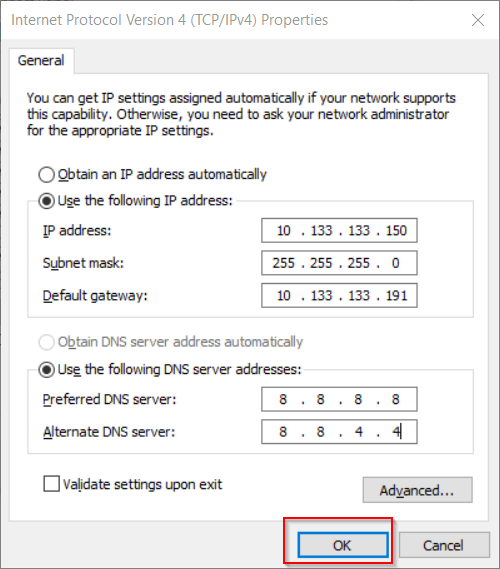
\includegraphics[width=1\textwidth]{images/5.5.png} 
    \label{fig:network}
    \end{figure}

\subsubsection{Step 6: Test Using Ping}
\begin{itemize}
    \item Open Command Prompt
    
    \item Run:
    \begin{verbatim}
ping 10.133.133.191
ping 8.8.8.8
ping google.com
    \end{verbatim}
    
    \item Reply received $\rightarrow$ Configuration is correct
    
    \item Request timed out $\rightarrow$ Check settings
\end{itemize}
    \begin{figure}[H]
    \centering
    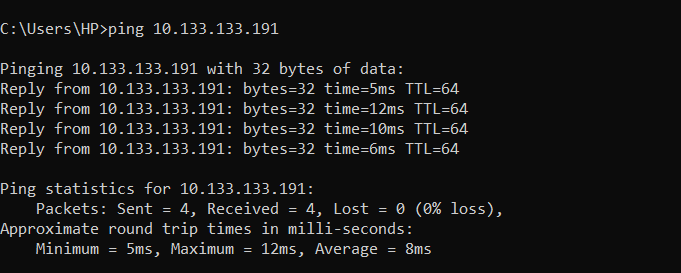
\includegraphics[width=1\textwidth]{images/5.6-1.png} 
    \label{fig:network}
    \end{figure}
        \begin{figure}[H]
    \centering
    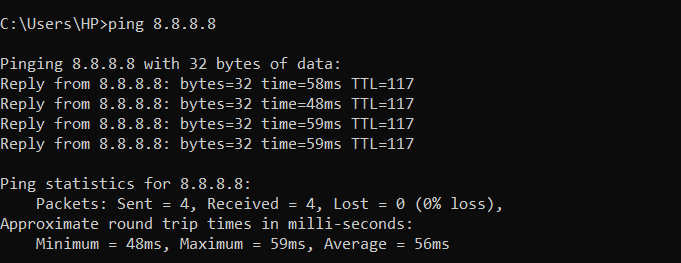
\includegraphics[width=1\textwidth]{images/5.6-2.png} 
    \label{fig:network}
    \end{figure}
        \begin{figure}[H]
    \centering
    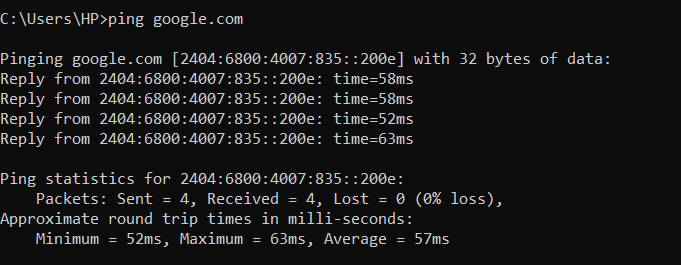
\includegraphics[width=1\textwidth]{images/5.6-3.png} 
    \label{fig:network}
    \end{figure}

\subsection{Observation:}
IP configuration was successful and connectivity verified.

\subsection{Viva Questions:}
\begin{enumerate}
    \item What is IP address?
    \item What is DNS?
\end{enumerate}

% -------------------- EXPERIMENT - 06 --------------------
\newpage
\section{EXPERIMENT - 06}
\subsection{Title:}
Study of Networking Devices

\subsection{Aim/Objective:}
To study various networking devices.

\subsection{Theory:}
Devices like repeater, hub, bridge, switch, router, gateway, access point, firewall, Network Interface Card (NIC) etc help in communication between devices.

\subsubsection{Repeater}
A repeater is a basic networking device that receives weak or degraded signals, regenerates them, and retransmits them to extend the distance of a network. It operates at the Physical Layer (Layer 1) of the OSI model and does not analyze or filter data—it simply boosts the signal strength. Repeaters are commonly used in both wired and wireless networks, such as Wi-Fi range extenders, to improve coverage in large areas.
    \begin{figure}[H]
    \centering
    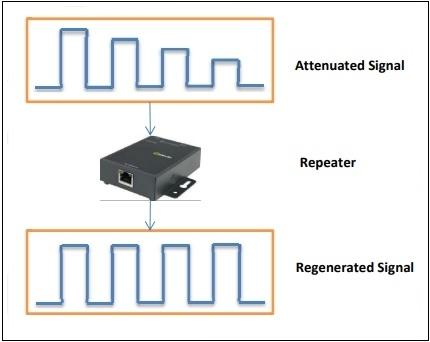
\includegraphics[width=0.7\textwidth]{images/6.1-1.jpg} 
    \caption{Repeater}
    \label{fig:network}
    \end{figure}
    \begin{figure}[H]
    \centering
    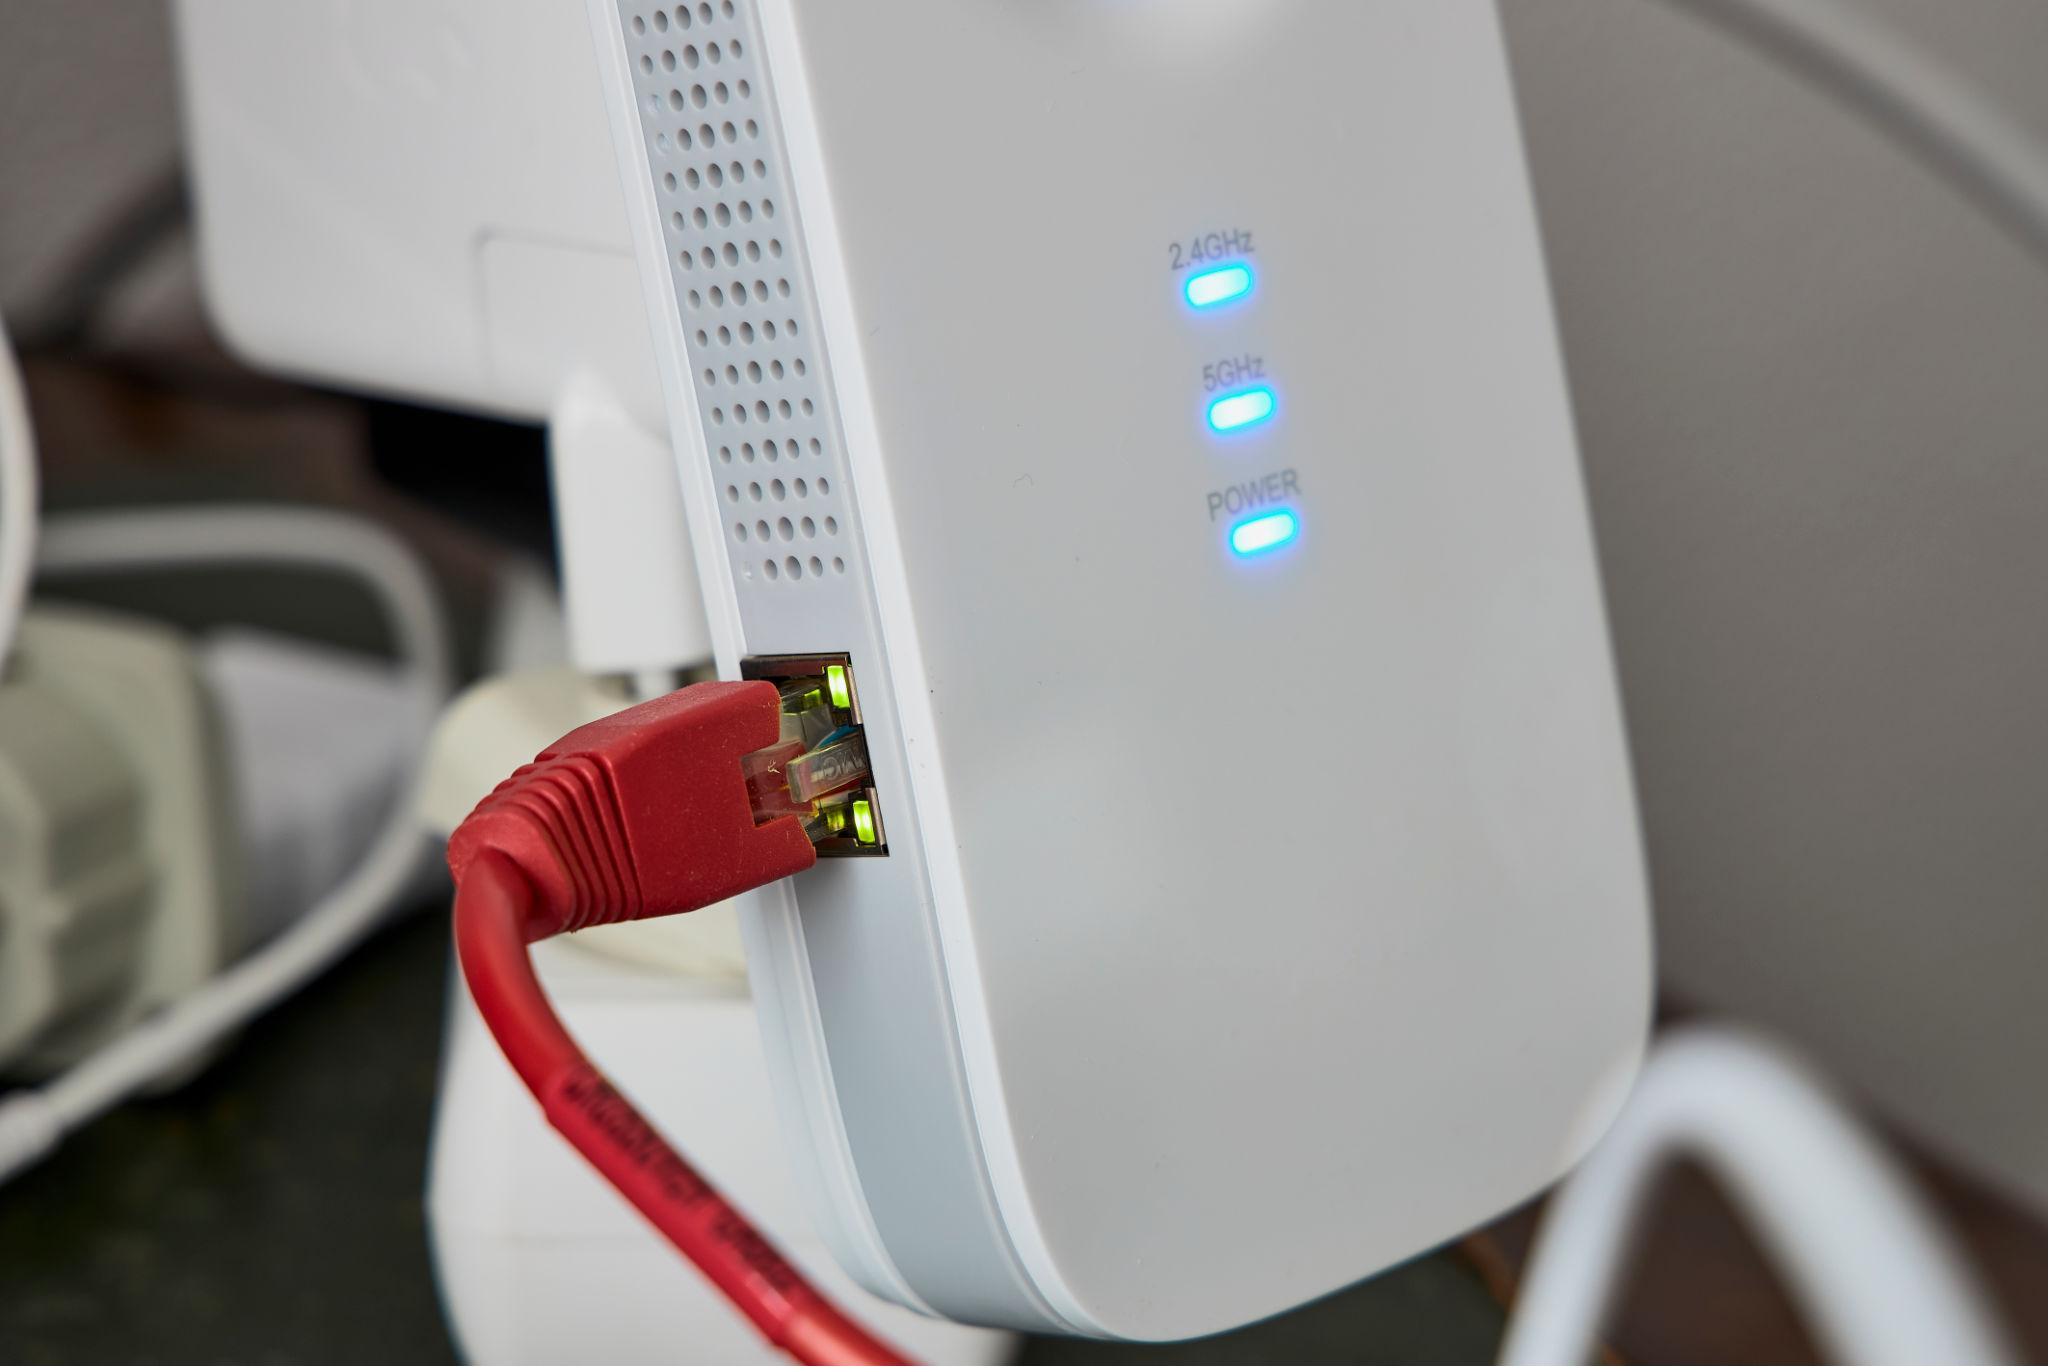
\includegraphics[width=0.7\textwidth]{images/6.1-2.jpg} 
    \caption{Repeater}
    \label{fig:network}
    \end{figure}
    \begin{figure}[H]
    \centering
    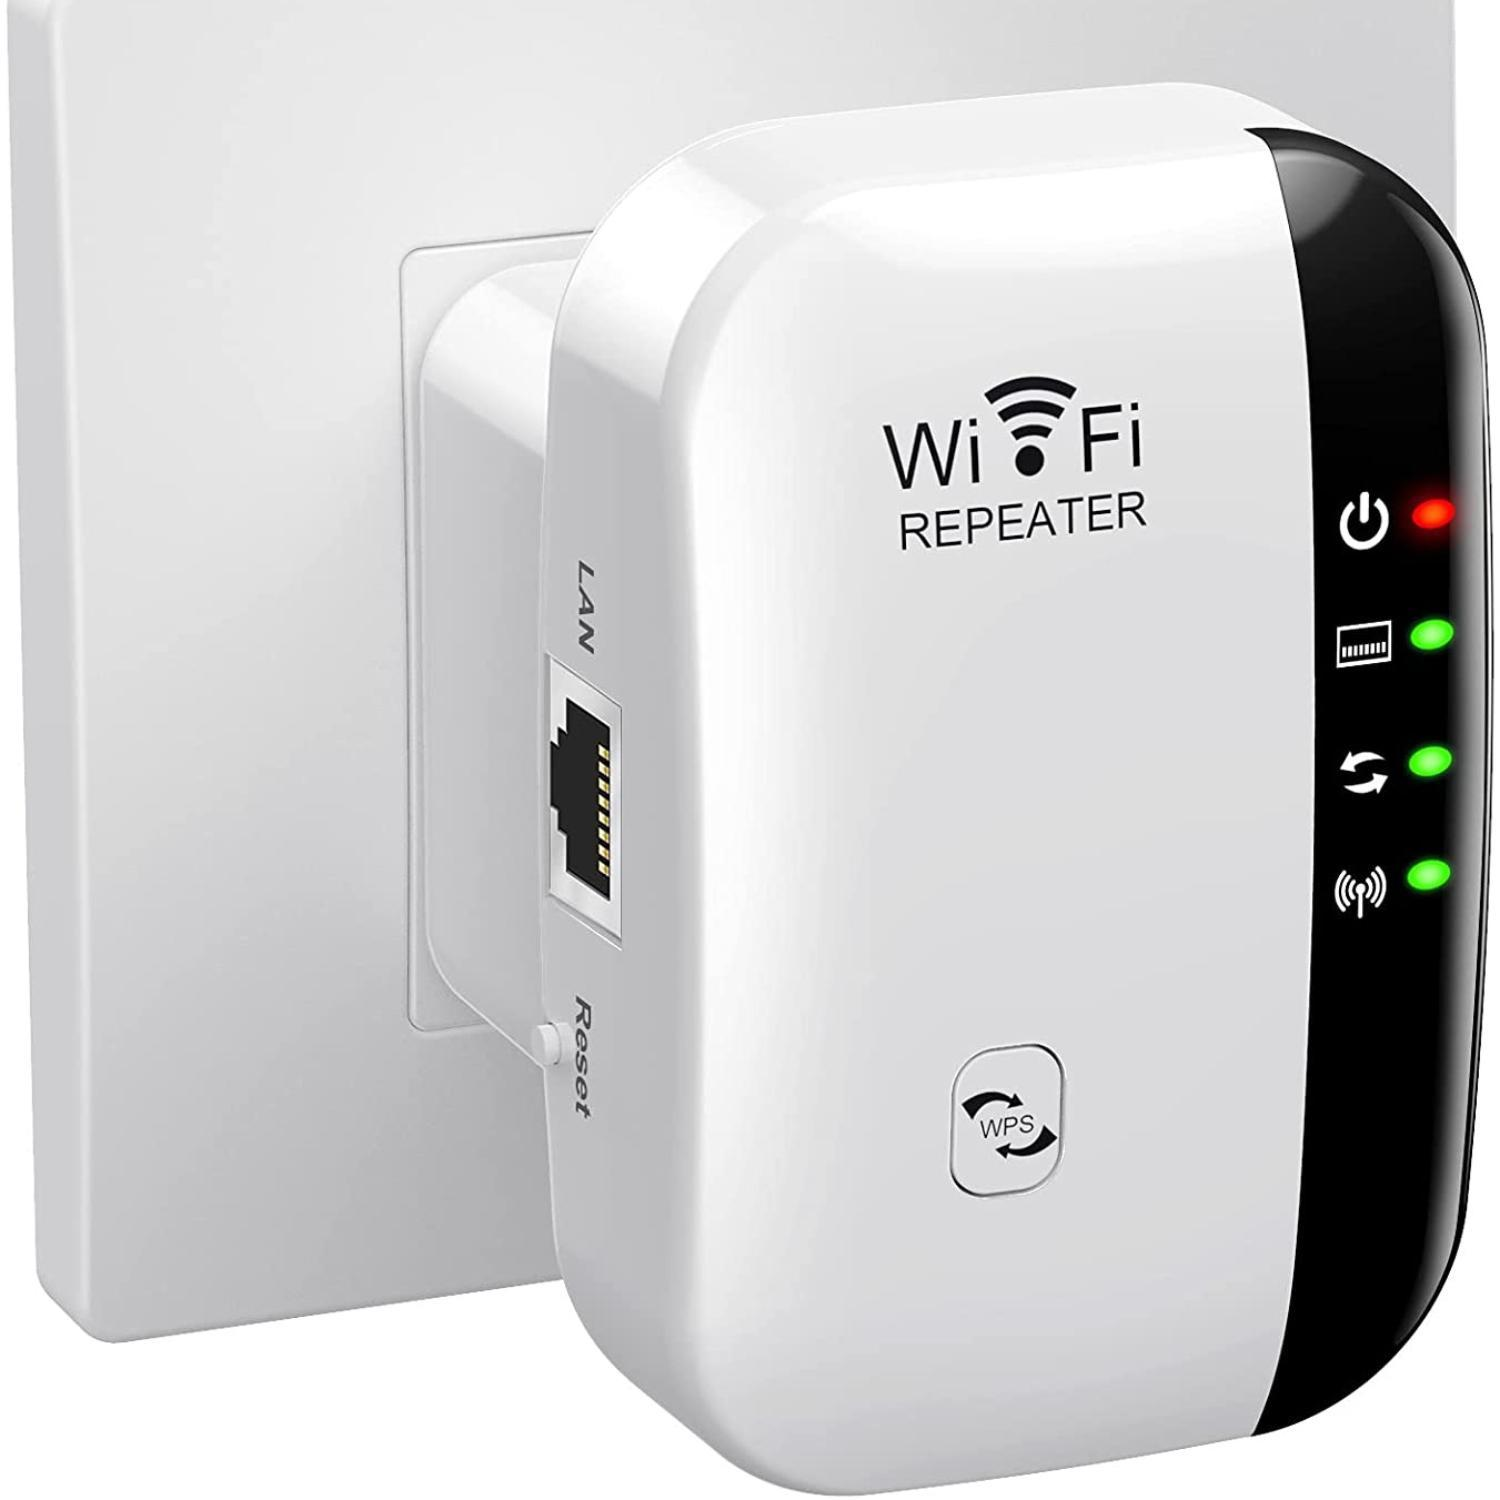
\includegraphics[width=0.7\textwidth]{images/6.1-3.jpg} 
    \caption{Repeater}
    \label{fig:network}
    \end{figure}

\subsubsection{Hub}
A hub is a basic networking device used to connect multiple computers in a local area network (LAN). It works at the Physical Layer (Layer 1) and simply broadcasts incoming data to all connected devices, without checking the destination address. Because of this, hubs are inefficient and can cause network congestion. They are now mostly outdated and have been replaced by switches, which provide smarter data transmission.
    \begin{figure}[H]
    \centering
    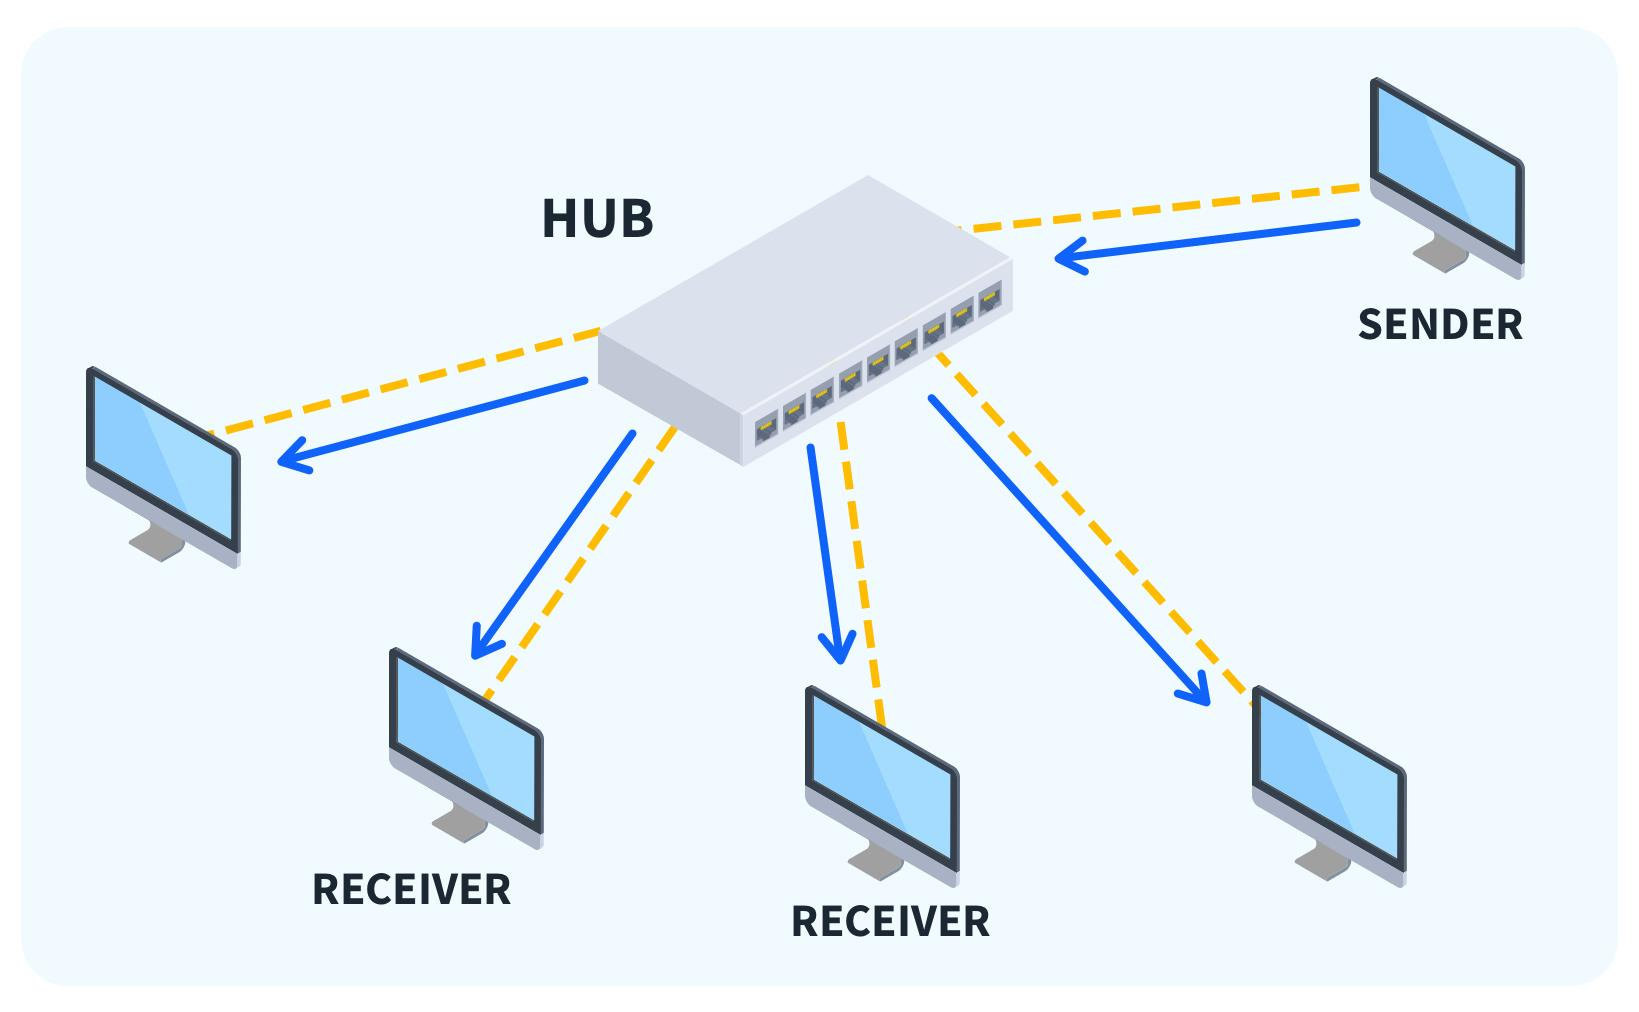
\includegraphics[width=0.7\textwidth]{images/6.2-1.jpg} 
    \caption{Hub}
    \label{fig:network}
    \end{figure}
    \begin{figure}[H]
    \centering
    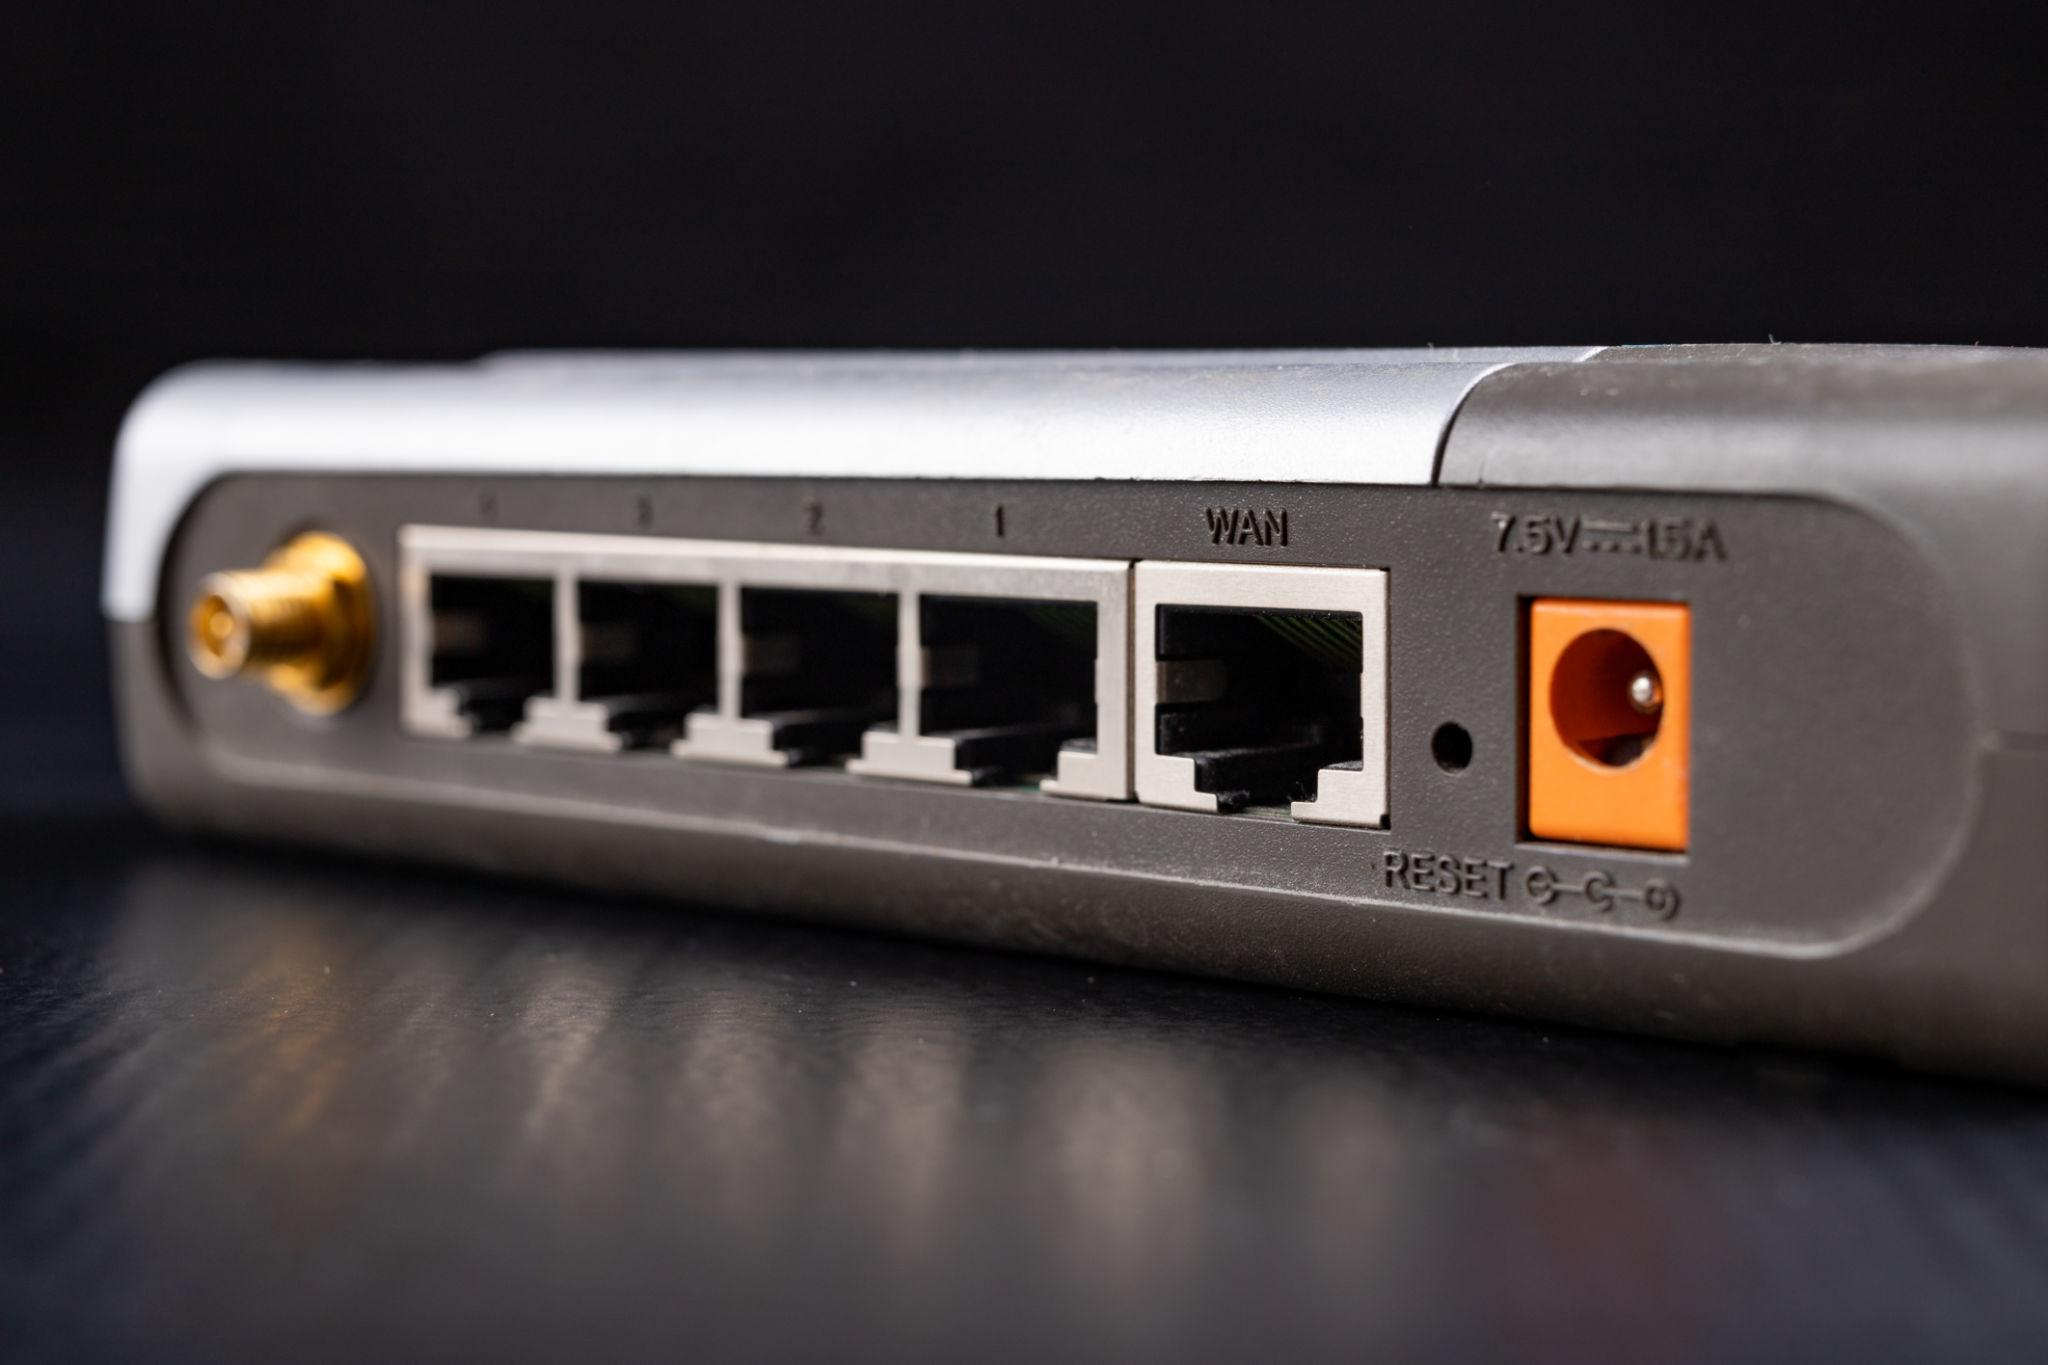
\includegraphics[width=0.7\textwidth]{images/6.2-2.jpg} 
    \caption{Hub}
    \label{fig:network}
    \end{figure}

\subsubsection{Bridge}
A bridge is a networking device that connects two or more LAN segments and controls data flow between them. It operates at the Data Link Layer (Layer 2) and uses MAC addresses to decide whether to forward or block traffic, helping reduce unnecessary data transmission. By segmenting a network, a bridge improves performance and minimizes collisions, making communication more efficient compared to hubs.
    \begin{figure}[H]
    \centering
    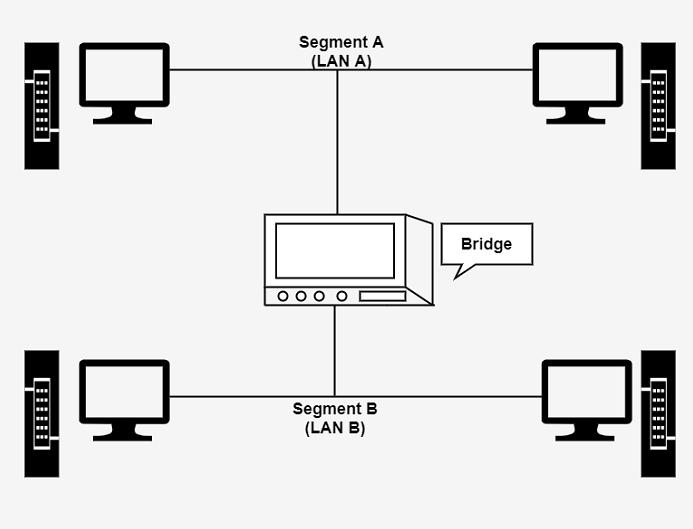
\includegraphics[width=0.7\textwidth]{images/6.3-1.jpg} 
    \caption{Bridge}
    \label{fig:network}
    \end{figure}

\subsubsection{Switch}
A switch is a networking device that connects multiple devices within a LAN and forwards data only to the intended recipient instead of broadcasting to all devices. It operates mainly at the Data Link Layer (Layer 2) and uses a MAC address table to intelligently direct traffic. This reduces network congestion and improves performance, making switches far more efficient than hubs in modern networks.
    \begin{figure}[H]
    \centering
    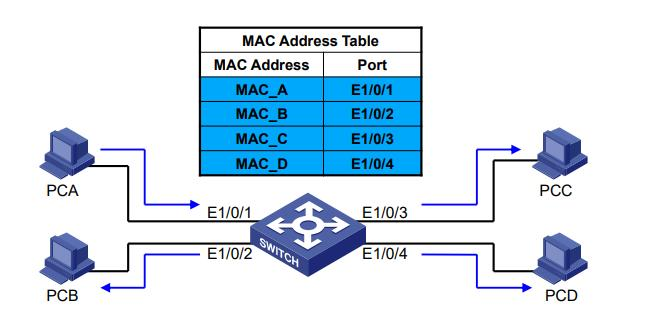
\includegraphics[width=0.7\textwidth]{images/6.4-1.jpg} 
    \caption{Switch}
    \label{fig:network}
    \end{figure}
    \begin{figure}[H]
    \centering
    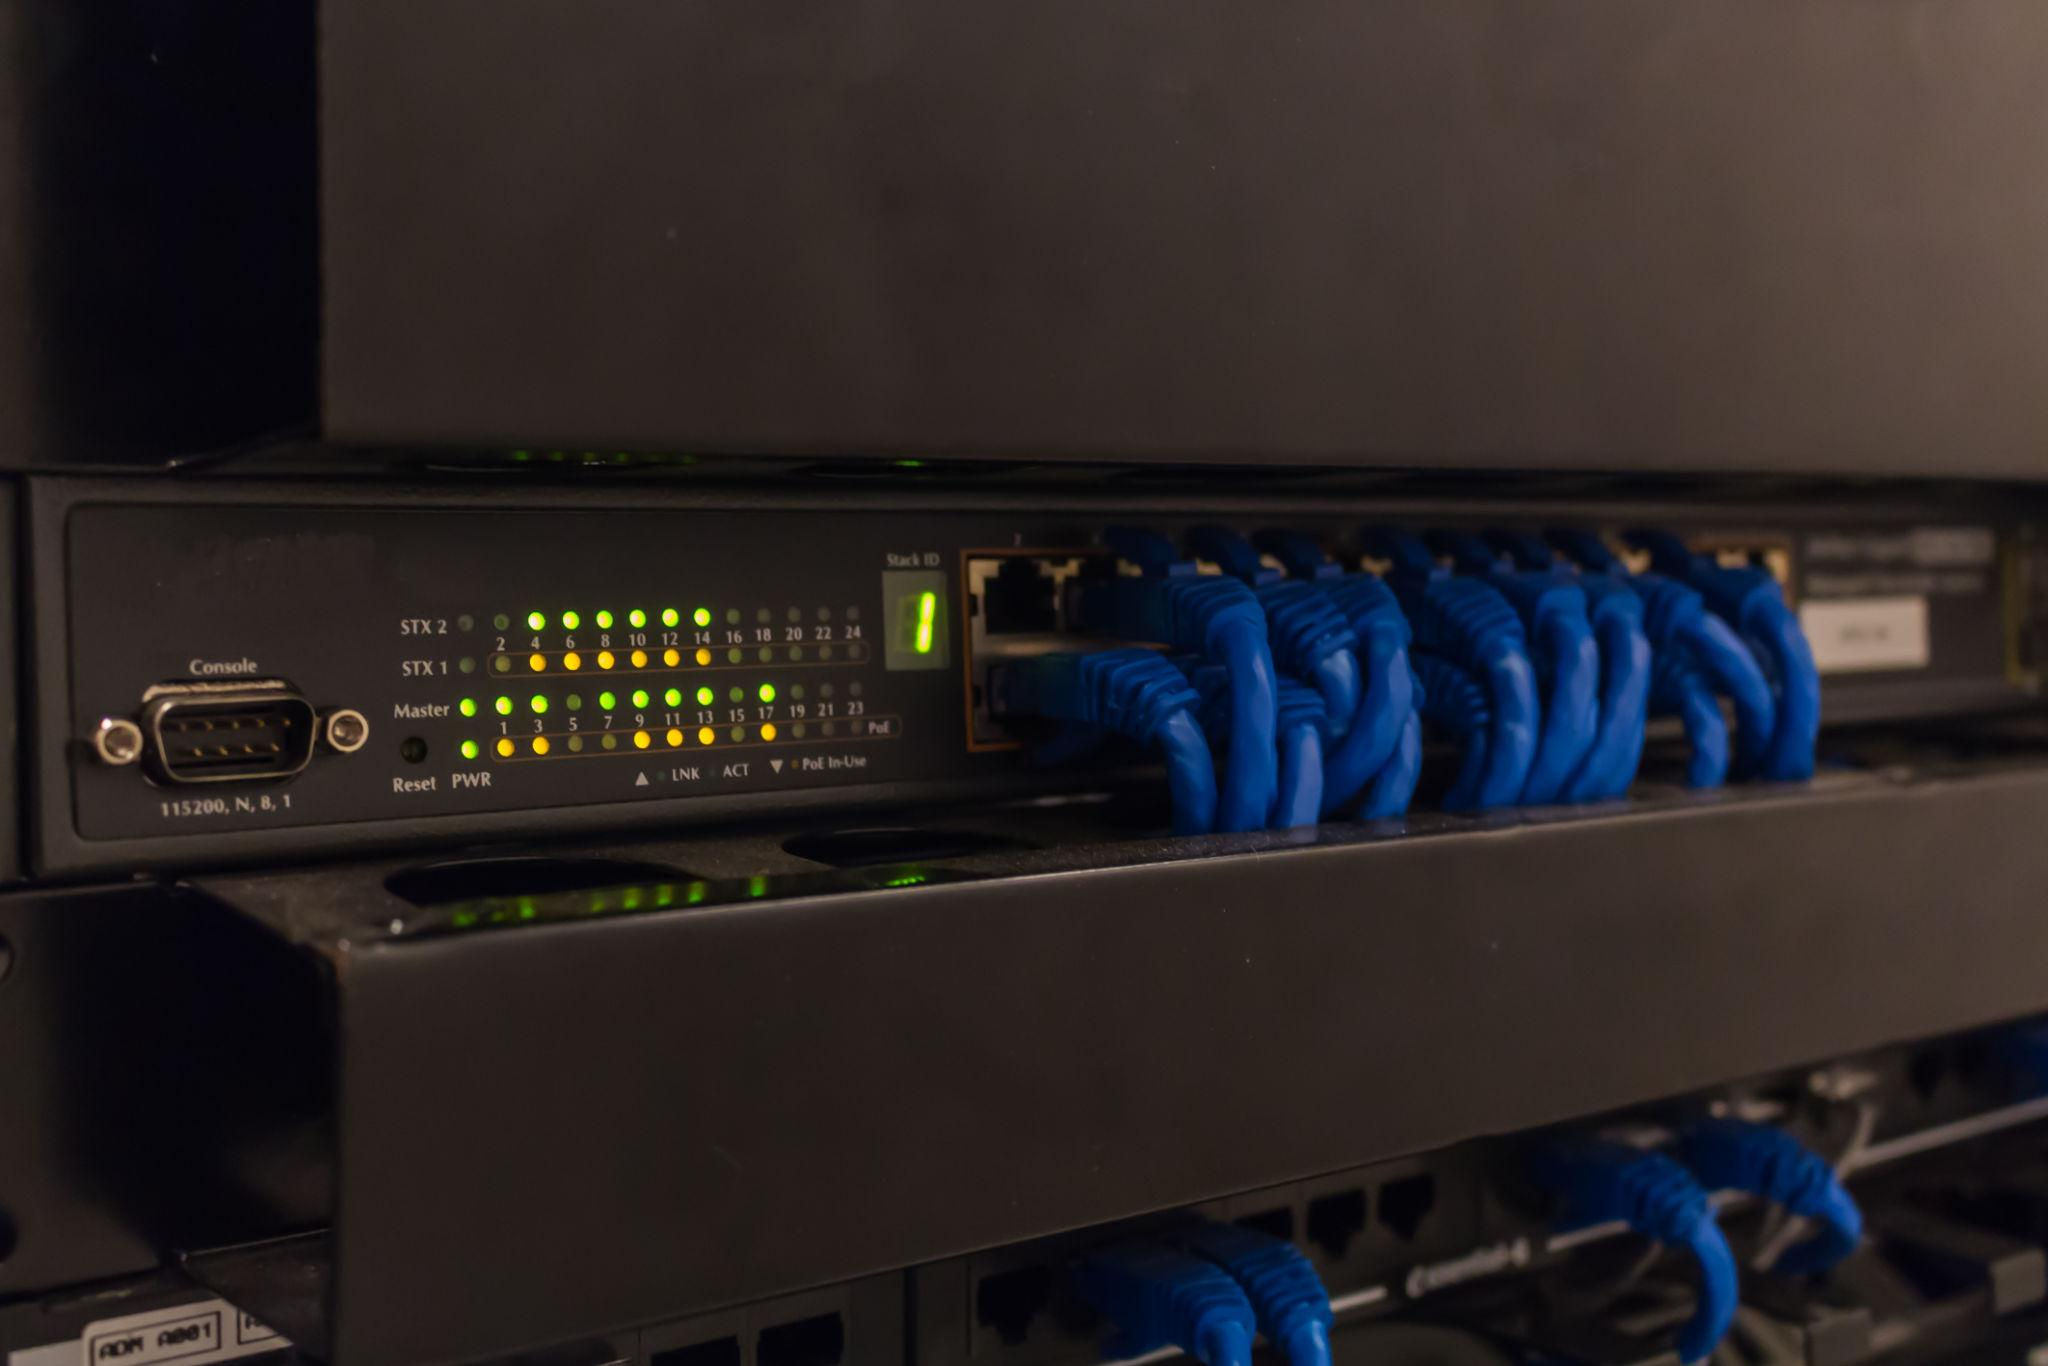
\includegraphics[width=0.7\textwidth]{images/6.4-2.jpg} 
    \caption{Switch}
    \label{fig:network}
    \end{figure}

\subsubsection{Router}
A router is a networking device that connects different networks, such as a local area network (LAN) to the internet, and forwards data packets based on IP addresses. It operates at the Network Layer (Layer 3) and determines the best path for data to travel between networks. Routers are commonly used in homes and offices to provide internet access and often include additional features like Wi-Fi and basic security.
    \begin{figure}[H]
    \centering
    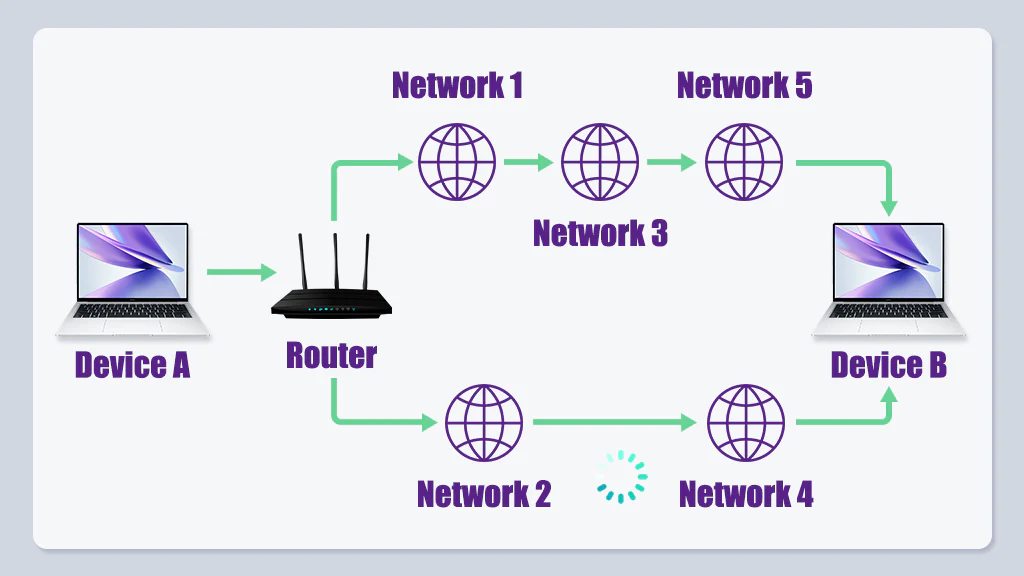
\includegraphics[width=0.7\textwidth]{images/6.5-1.jpg} 
    \caption{Router}
    \label{fig:network}
    \end{figure}
    \begin{figure}[H]
    \centering
    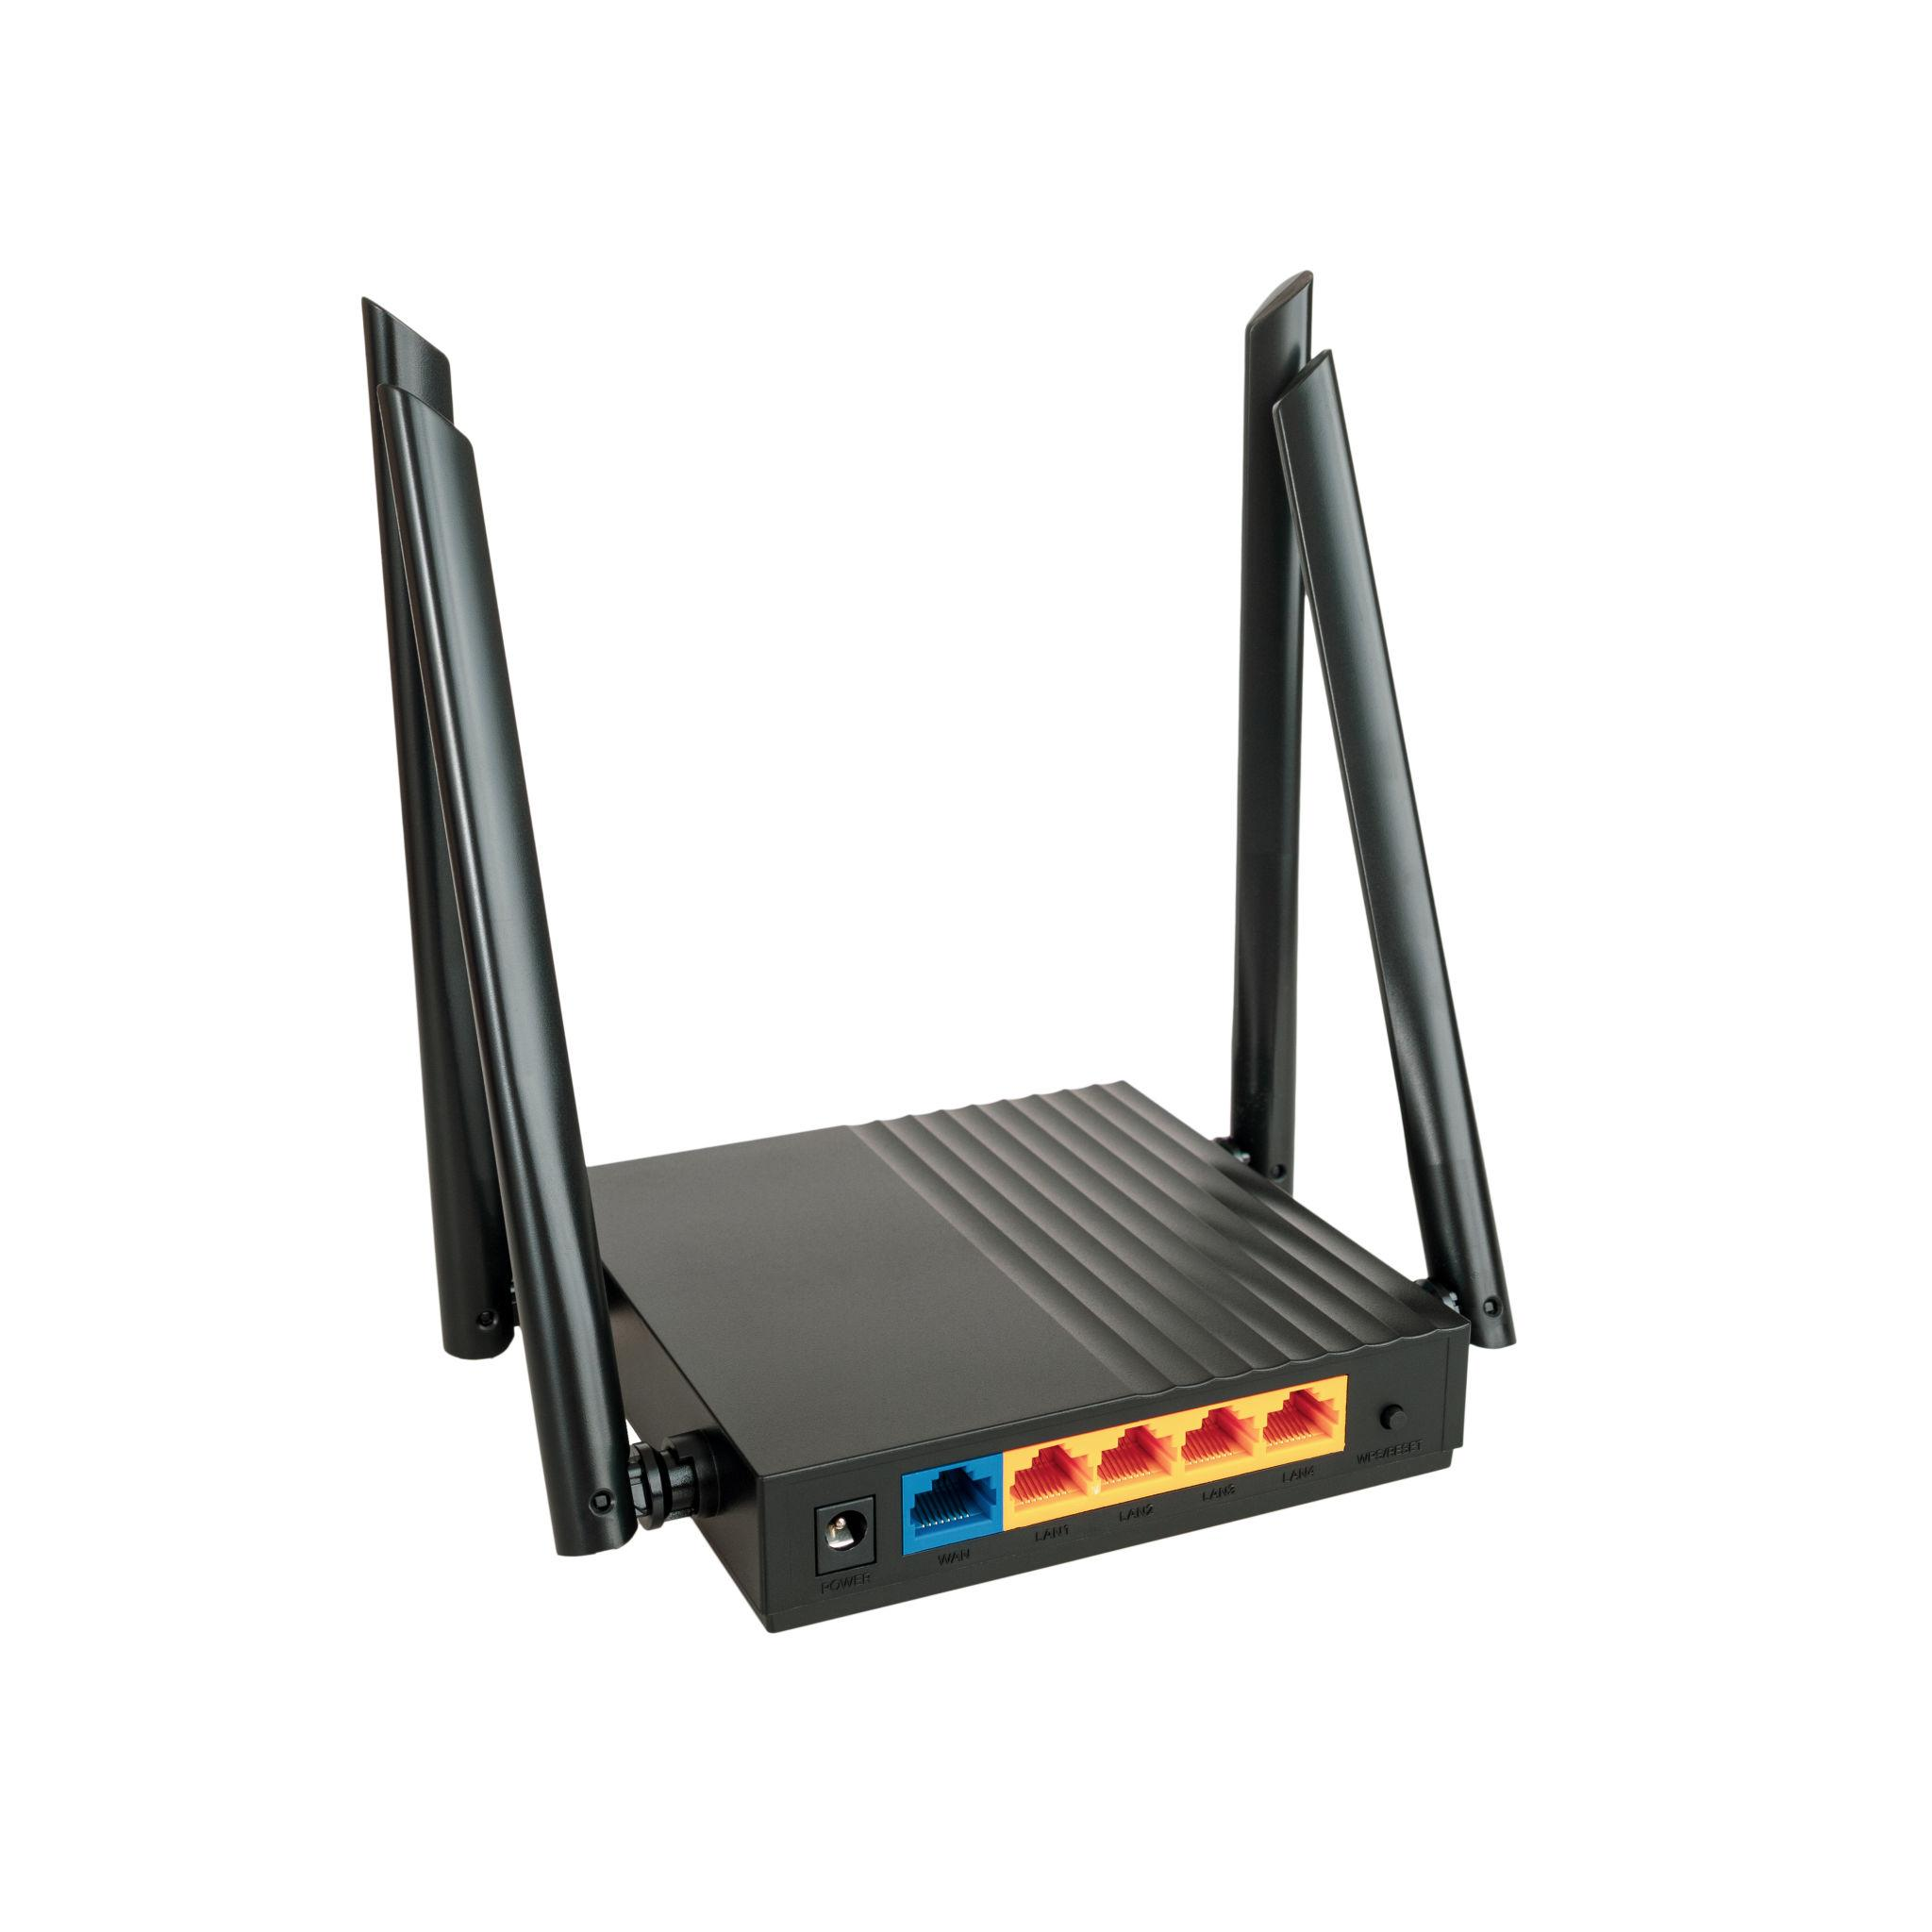
\includegraphics[width=0.7\textwidth]{images/6.5-2.jpg} 
    \caption{Router}
    \label{fig:network}
    \end{figure}

\subsubsection{Gateway}
A gateway is a networking device that acts as a bridge between different networks using different protocols, enabling them to communicate with each other. It operates across multiple layers of the OSI model and can perform tasks like protocol conversion, data translation, and routing. In most networks, the router also serves as the default gateway, allowing devices in a local network to access external networks like the internet.
    \begin{figure}[H]
    \centering
    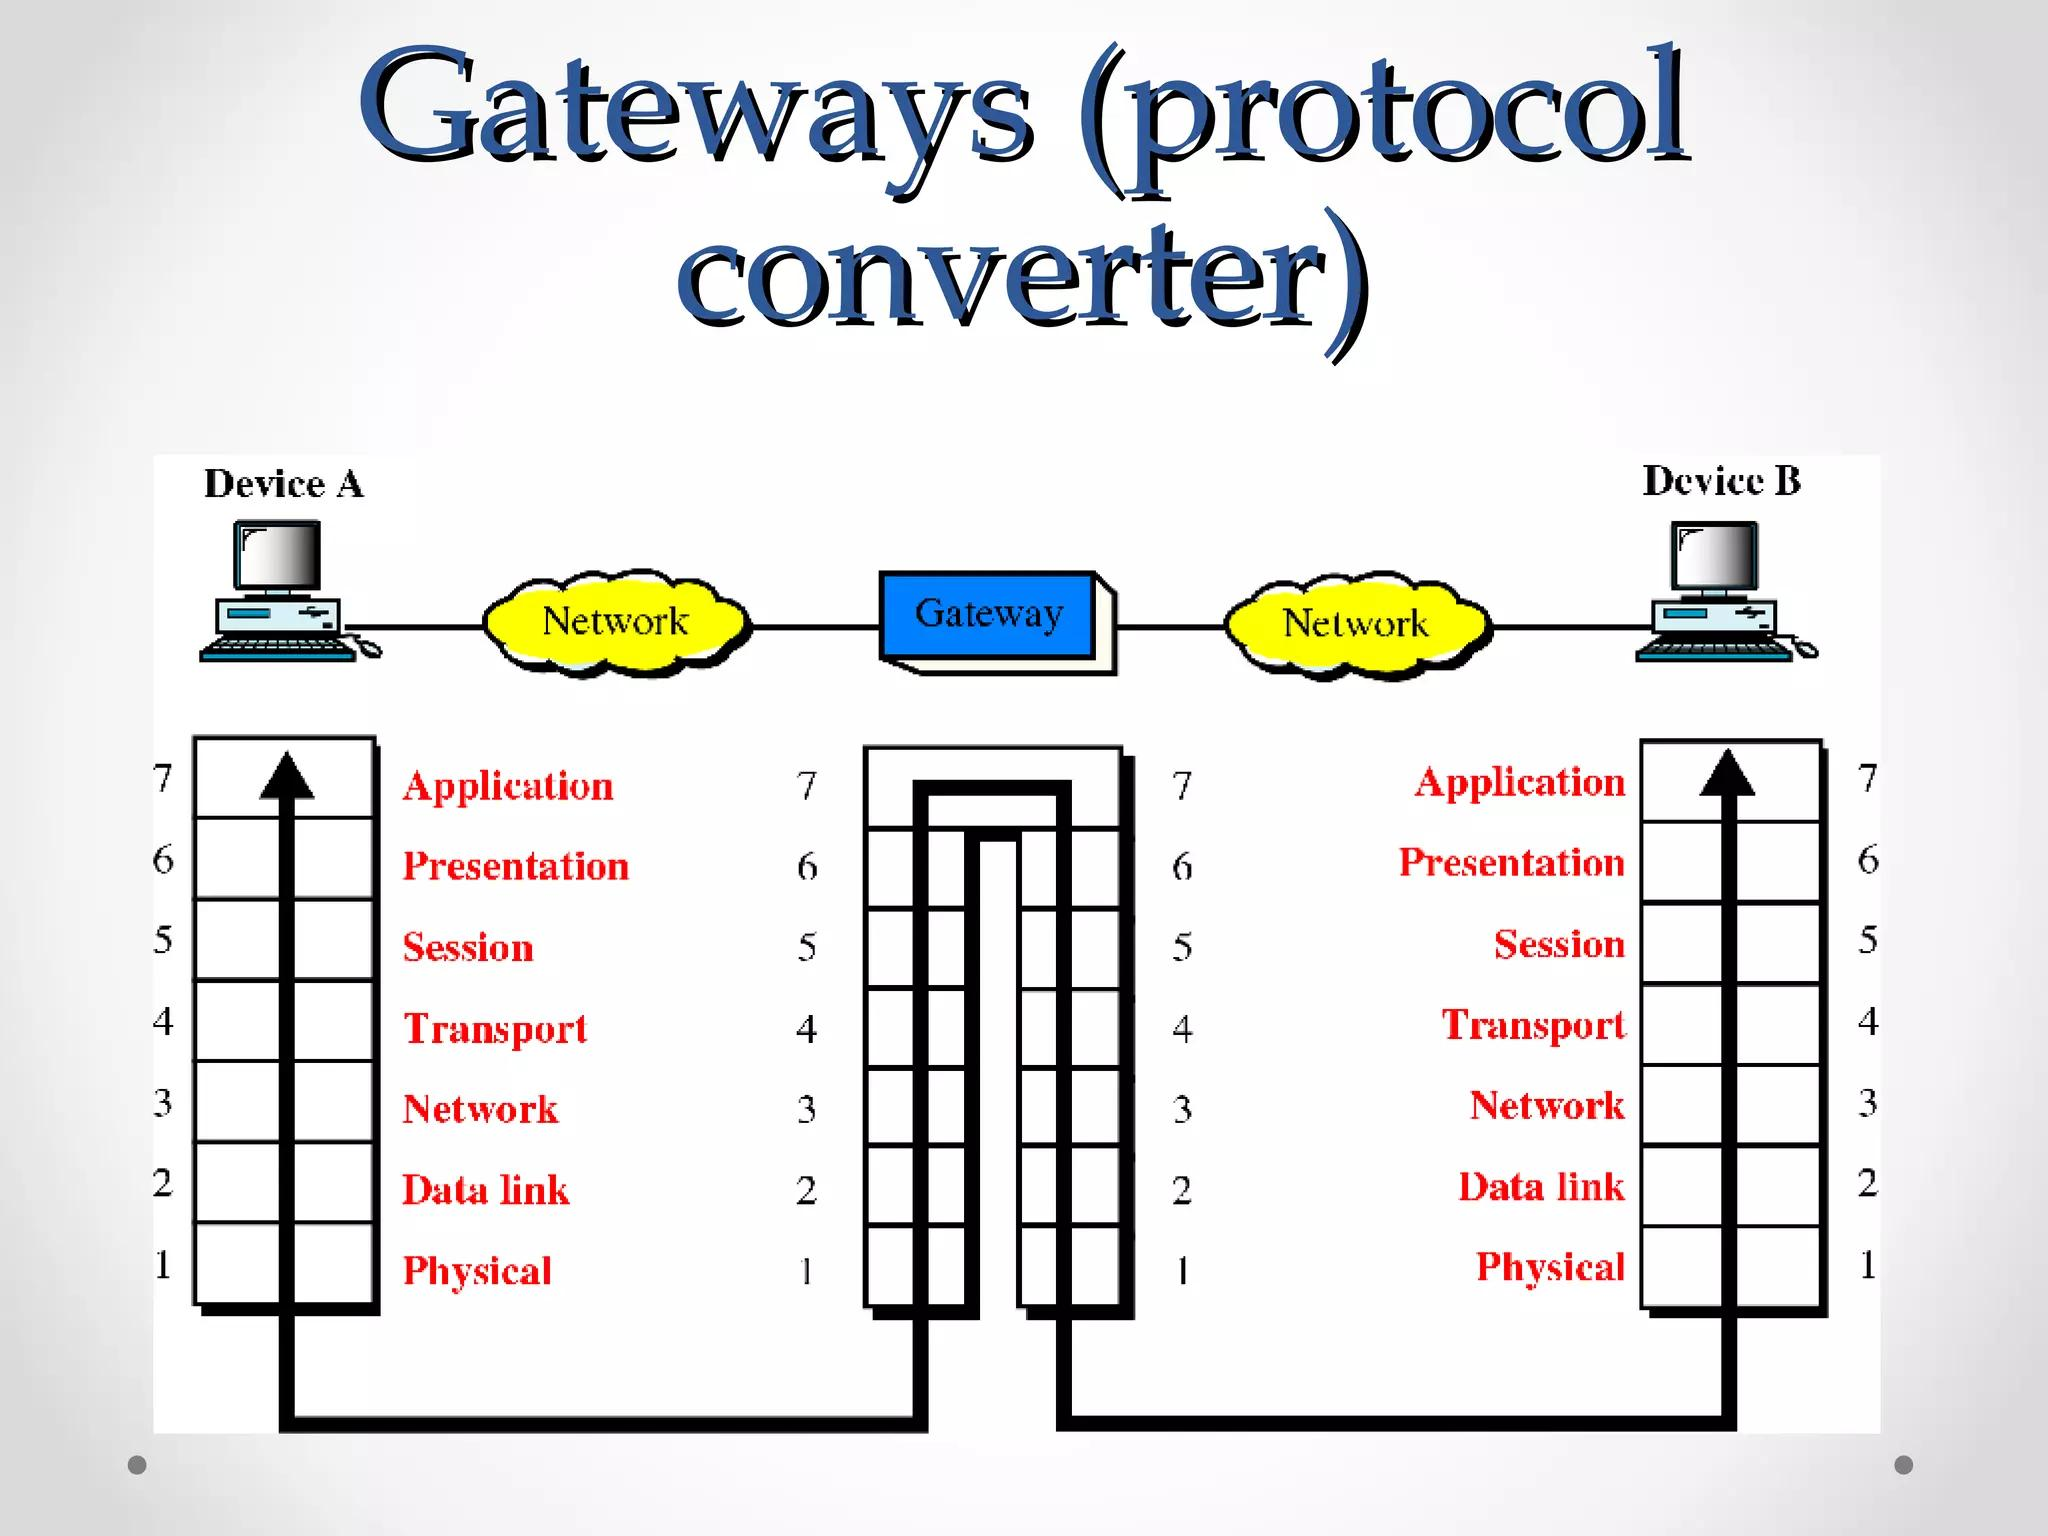
\includegraphics[width=0.6\textwidth]{images/6.6-1.jpg} 
    \caption{Gateway}
    \label{fig:network}
    \end{figure}
    \begin{figure}[H]
    \centering
    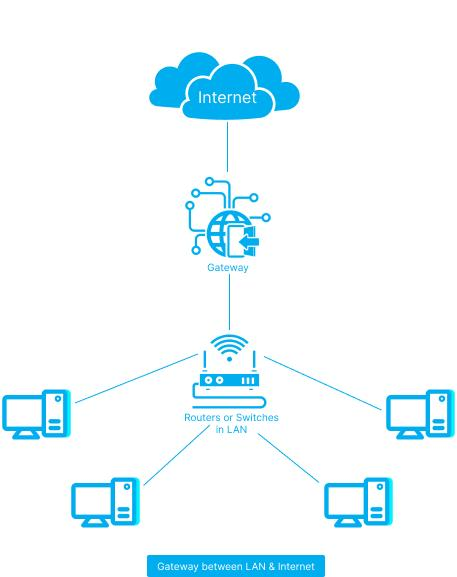
\includegraphics[width=0.6\textwidth]{images/6.6-2.jpg} 
    \caption{Gateway}
    \label{fig:network}
    \end{figure}

\subsubsection{Access Point (AP)}
An access point (AP) is a networking device that provides wireless connectivity by allowing Wi-Fi-enabled devices (like laptops and smartphones) to connect to a wired network. It operates mainly at the Data Link Layer (Layer 2) and acts as a bridge between wired and wireless networks. Access points are commonly used in homes, offices, and public spaces to extend Wi-Fi coverage and improve network accessibility.
    \begin{figure}[H]
    \centering
    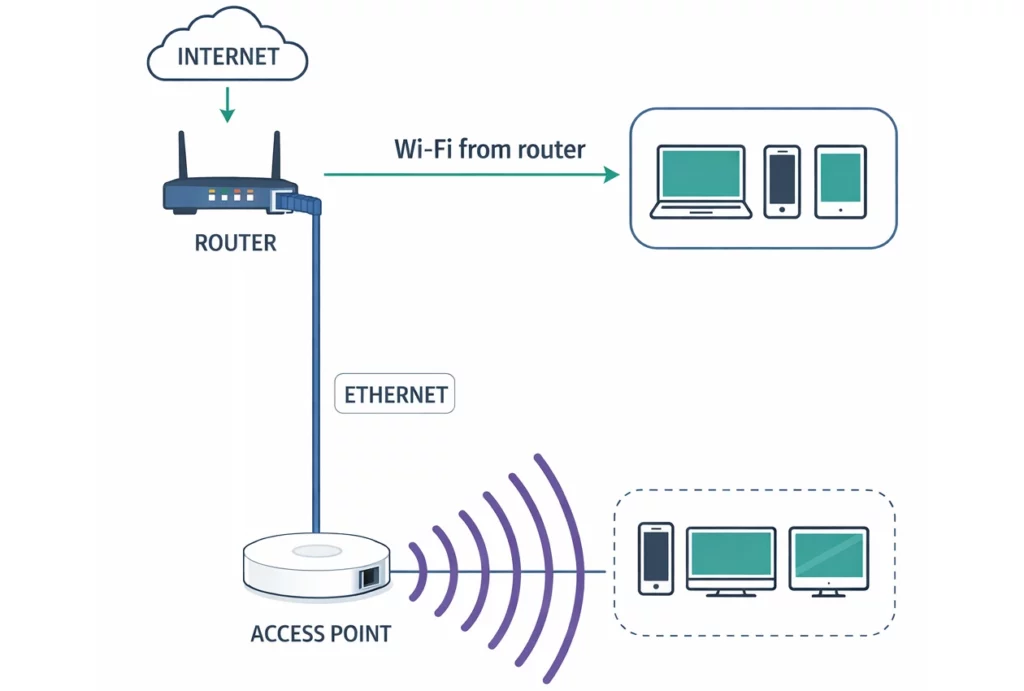
\includegraphics[width=0.6\textwidth]{images/6.7-2.jpg} 
    \caption{Access Point (AP)}
    \label{fig:network}
    \end{figure}
    \begin{figure}[H]
    \centering
    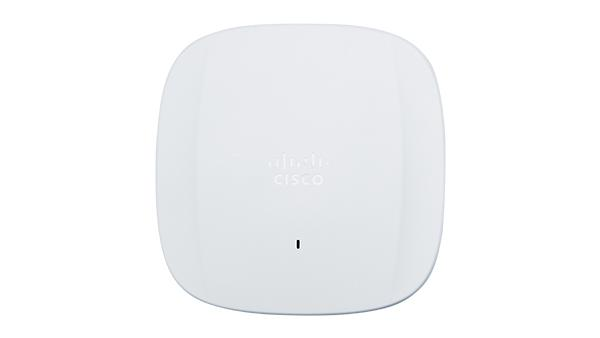
\includegraphics[width=0.7\textwidth]{images/6.7-1.jpg} 
    \caption{Access Point (AP)}
    \label{fig:network}
    \end{figure}

\subsubsection{Firewall}
A firewall is a network security device that monitors and controls incoming and outgoing traffic based on predefined security rules. It helps protect networks from unauthorized access, cyberattacks, and malware by allowing or blocking data packets. Firewalls can be hardware-based or software-based and operate across multiple layers of the OSI model, ensuring safe communication between internal and external networks.
    \begin{figure}[H]
    \centering
    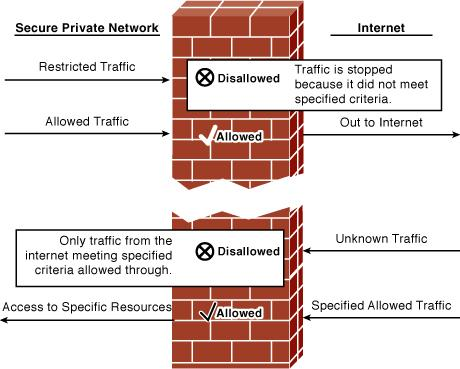
\includegraphics[width=0.6\textwidth]{images/6.8-1.jpg} 
    \caption{Firewall}
    \label{fig:network}
    \end{figure}
    \begin{figure}[H]
    \centering
    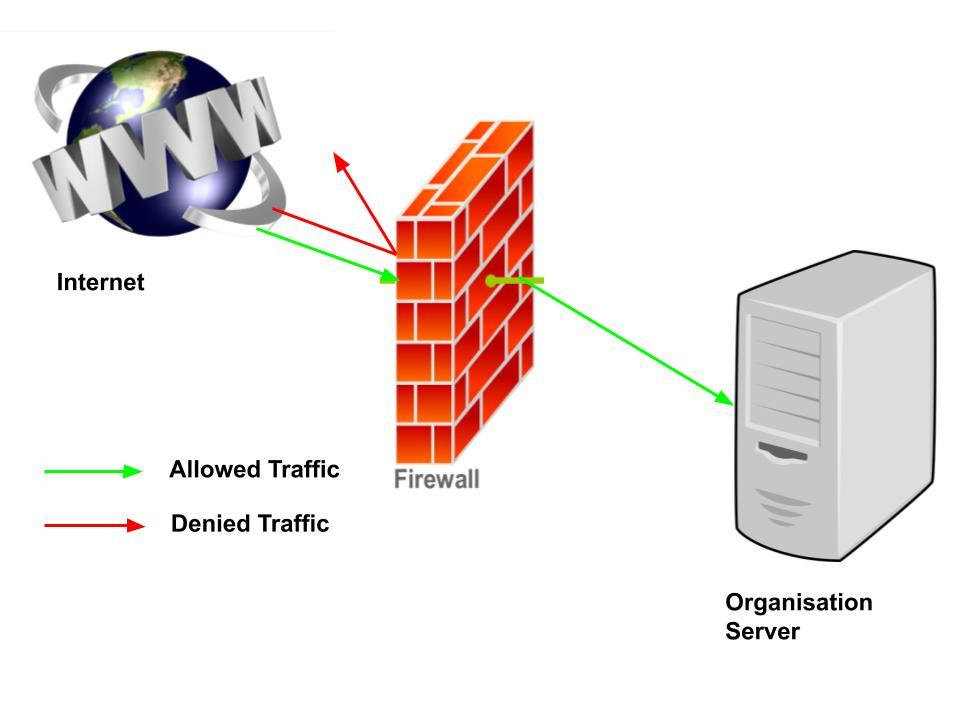
\includegraphics[width=0.7\textwidth]{images/6.8-2.jpg} 
    \caption{Firewall}
    \label{fig:network}
    \end{figure}
    \begin{figure}[H]
    \centering
    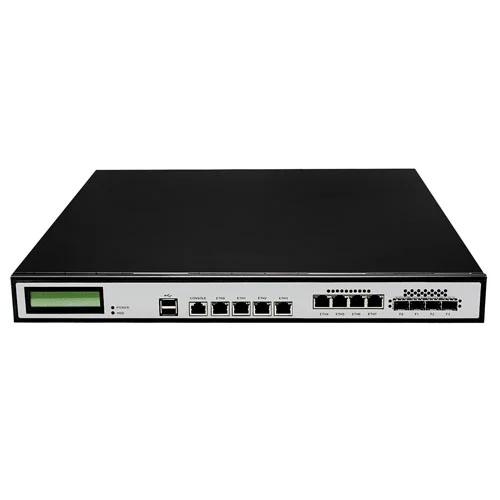
\includegraphics[width=0.7\textwidth]{images/6.8-3.jpg} 
    \caption{Firewall}
    \label{fig:network}
    \end{figure}

\subsubsection{Network Interface Card (NIC)}
A Network Interface Card (NIC) is a hardware component that connects a computer or device to a network. It can be wired (Ethernet) or wireless (Wi-Fi) and provides a unique MAC address used for identification in a network. The NIC operates mainly at the Data Link Layer (Layer 2) and enables devices to send and receive data over the network.
    \begin{figure}[H]
    \centering
    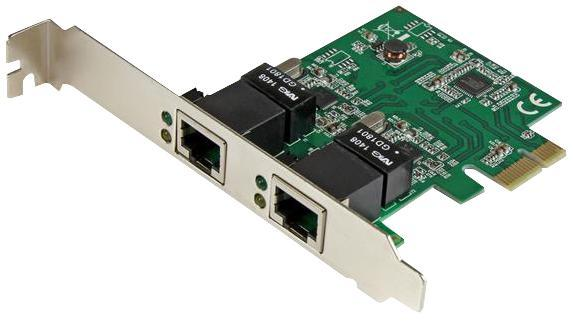
\includegraphics[width=0.6\textwidth]{images/6.9-1.jpg} 
    \caption{Network Interface Card (NIC)}
    \label{fig:network}
    \end{figure}
    \begin{figure}[H]
    \centering
    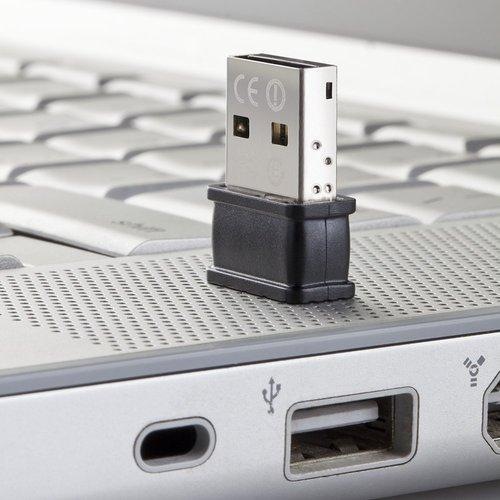
\includegraphics[width=0.7\textwidth]{images/6.9-2.jpg} 
    \caption{Network Interface Card (NIC)}
    \label{fig:network}
    \end{figure}
    
\subsection{Apparatus/Equipments/Softwares:}
\begin{itemize}
    \item Repeater
    \item Hub
    \item Bridge
    \item Switch
    \item Router
    \item Gateway
    \item Access Point (AP)
    \item Firewall
    \item Network Interface Card (NIC)
\end{itemize}

\subsection{Procedure:}
\begin{enumerate}
    \item Observe devices
    \item Note their functions
\end{enumerate}

\subsection{Observation:}
Different networking devices and their uses were understood.

\subsection{Viva Questions:}
\begin{enumerate}
    \item What is router?
    \item Difference between hub and switch?
\end{enumerate}

% -------------------- EXPERIMENT - 07 --------------------
\newpage
\section{EXPERIMENT - 07}
\subsection{Title:}
Comparison of Networking Devices

\subsection{Aim/Objective:}
To compare the specifications, working, and features of different networking devices such as Repeater, Hub, Switch, Bridge, Router, and Gateway.

\subsection{Theory:}
Networking devices are used to connect computers and manage communication in a network.

Each device works at a different OSI layer and performs a specific function.
\begin{itemize}
    \item \textbf{Repeater \& Hub:} Work at Physical Layer (signal transmission)
    \item \textbf{Switch \& Bridge:} Work at Data Link Layer (MAC-based forwarding)
    \item \textbf{Router:} Works at Network Layer (IP-based routing)
    \item \textbf{Gateway:} Works across all layers (protocol conversion)
\end{itemize}

These devices differ in:
\begin{itemize}
    \item Speed
    \item Intelligence
    \item Addressing method
    \item Functionality
\end{itemize}

\subsection{Apparatus/Equipments/Softwares:}
\begin{itemize}
    \item Internet
    \item Computer System
\end{itemize}

\subsection{Procedure:}
\begin{enumerate}
    \item Search different networking devices on the Internet
    
    \item Study their:
    \begin{itemize}
        \item Working principle
        \item OSI layer
        \item Features
    \end{itemize}
    
    \item Compare their specifications
    
    \item Prepare a comparison table
    
    \item Analyze differences
\end{enumerate}

\subsection{Observation:}
\begin{table}[H]
\centering
\begin{tabular}{|c|c|c|c|c|c|}
\hline
\textbf{Device} & \textbf{Layer} & \textbf{Address Used} & \textbf{Speed} & \textbf{Ports} & \textbf{Function} \\
\hline
Repeater & L1 & None & Low & 2 & Regenerates signal \\
Hub & L1 & None & Low & Multiple & Broadcasts data \\
Bridge & L2 & MAC & Medium & 2--4 & Connects LAN segments \\
Switch & L2 & MAC & High & 24/48 & Forwards frames efficiently \\
Router & L3 & IP & High & 2--8 & Connects networks \\
Gateway & All & Any & Variable & Multiple & Protocol conversion \\
\hline
\end{tabular}
\caption{Comparison of Networking Devices}
\label{tab:network_devices}
\end{table}

\begin{itemize}
    \item Devices differ in speed and intelligence
    \item Switch is faster than Hub because it sends data to a specific device
    \item Router connects different networks, unlike switch
    \item Gateway acts as a translator between different protocols
\end{itemize}

\subsection{Viva Questions:}
\begin{enumerate}
    \item What is throughput?
    \item What is latency?
\end{enumerate}

% -------------------- EXPERIMENT - 08 --------------------
\newpage
\section{EXPERIMENT - 08}
\subsection{Title:}
Network Simulation using Packet Tracer

\subsection{Aim/Objective:}
To simulate a computer network using software and test connectivity between devices.

\subsection{Theory:}
Network simulation is the process of designing and testing a network virtually using software tools. It helps in understanding how devices communicate without needing real hardware.

Cisco Packet Tracer is widely used for:
\begin{itemize}
    \item Designing network topologies
    \item Configuring devices (router, switch, PC)
    \item Testing connectivity using commands like ping
\end{itemize}
Advantages:
\begin{itemize}
    \item Cost-effective
    \item Safe environment
    \item Easy to modify
\end{itemize}
    
\subsection{Apparatus/Equipments/Softwares:}
\begin{itemize}
    \item Computer System
    \item Cisco Packet Tracer
\end{itemize}

\subsection{Procedure:}
\begin{enumerate}
    \item Open Cisco Packet Tracer
    
    \item Drag and drop devices:
    \begin{itemize}
        \item PCs
        \item Switch / Router
    \end{itemize}
    
    \item Connect devices using appropriate cables
    
    \item Assign IP addresses to each device
    
    \item Configure router (if used)
    
    \item Open Command Prompt on PC
    
    \item Use \texttt{ping} command to test connectivity
\end{enumerate}

\subsection{Practical Setup:}
\subsubsection{Topology:}
\begin{itemize}
    \item 2 PCs + 1 Switch
\end{itemize}
    \begin{figure}[H]
    \centering
    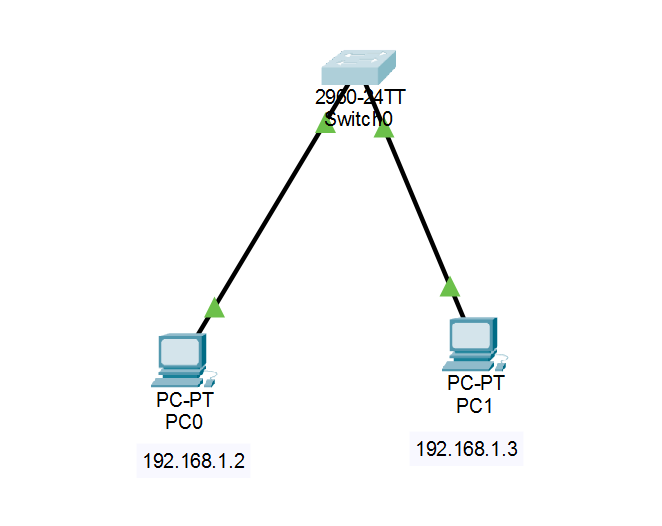
\includegraphics[width=0.7\textwidth]{images/8.1.png} 
    \caption{Topology}
    \label{fig:network}
    \end{figure}
\subsubsection{IP Configuration:}
\begin{itemize}
    \item PC1: \texttt{192.168.1.2}
    \item PC2: \texttt{192.168.1.3}
    \item Subnet Mask: \texttt{255.255.255.0}
\end{itemize}
    \begin{figure}[H]
    \centering
    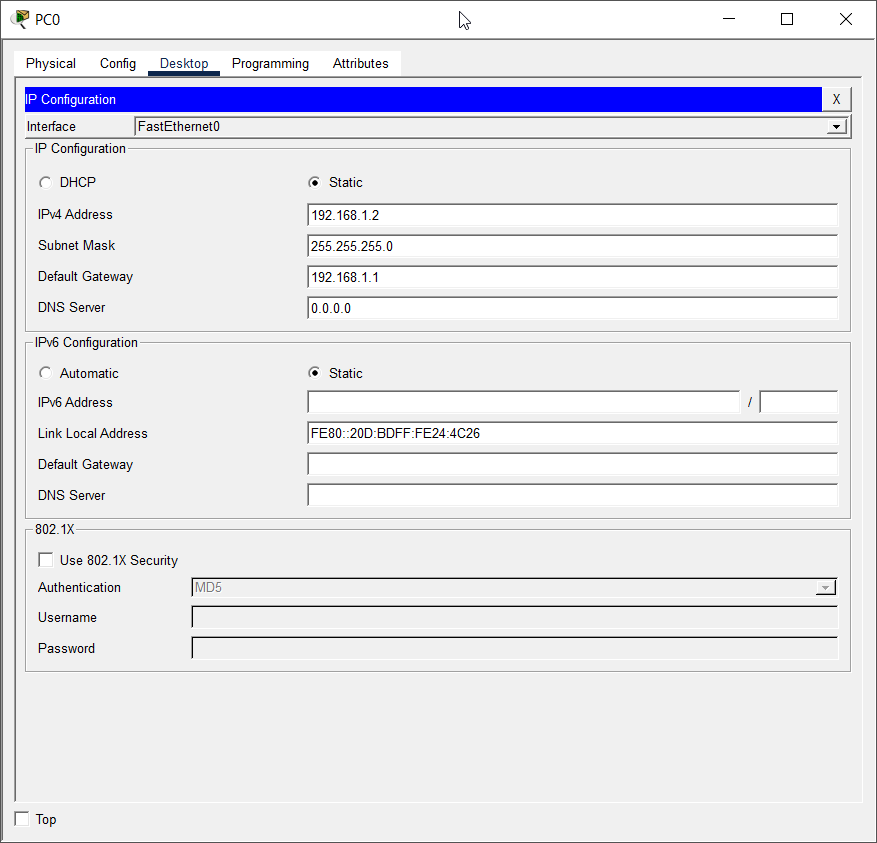
\includegraphics[width=1\textwidth]{images/8.2-1.png} 
    \caption{IP Address Configuration of PC0}
    \label{fig:network}
    \end{figure}
    \begin{figure}[H]
    \centering
    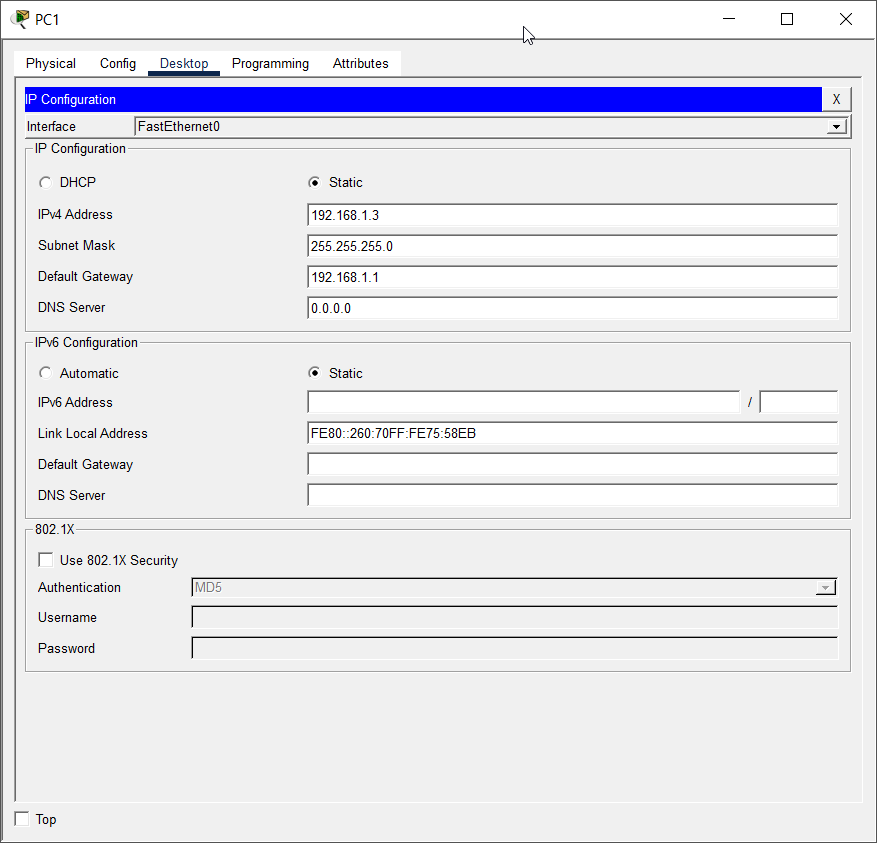
\includegraphics[width=1\textwidth]{images/8.2-2.png} 
    \caption{IP Address Configuration of PC1}
    \label{fig:network}
    \end{figure}
\subsubsection{Connectivity Test:}
On PC1:
\begin{lstlisting}
ping 192.168.1.2
\end{lstlisting}
    \begin{figure}[H]
    \centering
    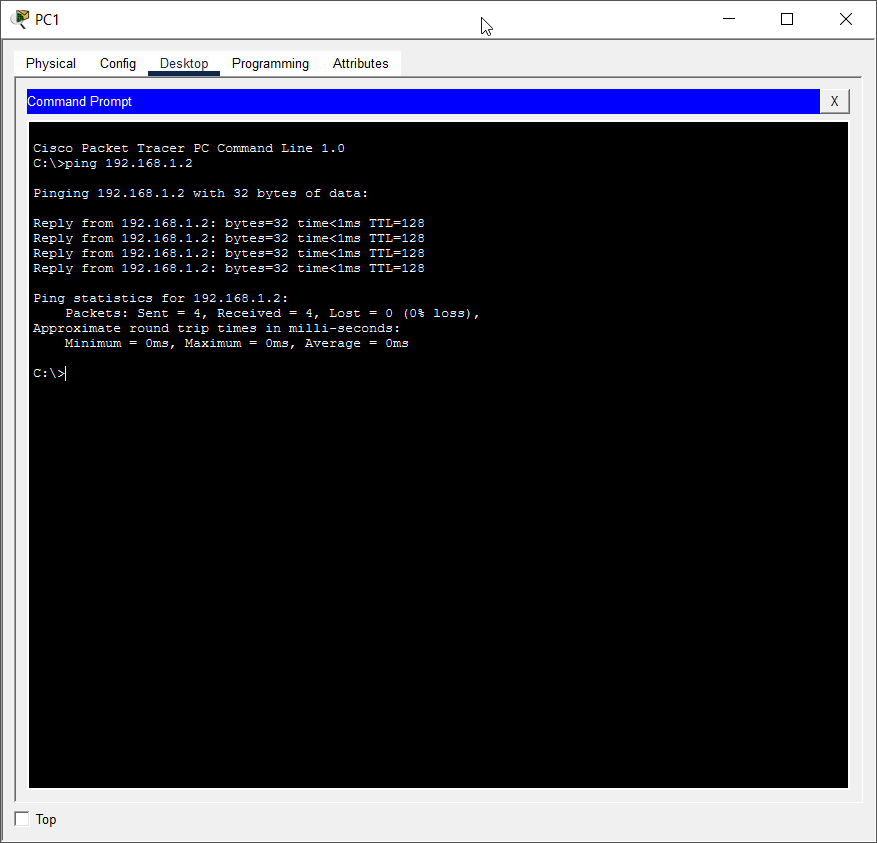
\includegraphics[width=1\textwidth]{images/8.3.png} 
    \caption{Network testing}
    \label{fig:network}
    \end{figure}
    
\subsection{Observation:}
\begin{itemize}
    \item Devices were successfully connected
    \item IP addresses were assigned correctly
    \item Ping test was successful
    \item Network simulation completed successfully
\end{itemize}

\subsection{Viva Questions:}
\begin{enumerate}
    \item What is simulation?
    \item Why use Packet Tracer?
\end{enumerate}

% -------------------- EXPERIMENT - 09 --------------------
\newpage
\section{EXPERIMENT - 09}
\subsection{Title:}
Setup of Wired LAN

\subsection{Aim/Objective:}
To create and configure a Wired Local Area Network (LAN) using switches and PCs.

\subsection{Theory:}
A Local Area Network (LAN) connects multiple devices within a limited area such as a lab, office, or home. In a wired LAN, devices are connected using Ethernet cables and communicate through a switch.
\begin{itemize}
    \item The switch forwards data using MAC addresses
    \item Communication is fast and secure compared to wireless
    \item Used in schools, offices, and labs
\end{itemize}
    
\subsection{Apparatus/Equipments/Softwares:}
\begin{itemize}
    \item PCs (2 or more)
    \item Network Switch
    \item LAN Cables (Ethernet – Straight-through)
    \item Cisco Packet Tracer
\end{itemize}

\subsection{Procedure:}
\begin{enumerate}
    \item Open Cisco Packet Tracer
    
    \item Drag and place:
    \begin{itemize}
        \item 1 Switch
        \item 2--4 PCs
    \end{itemize}
    
    \item Connect each PC to the switch using Copper Straight-through cable
    
    \item Assign IP addresses to each PC
    
    \item Open Command Prompt on PC
    
    \item Use \texttt{ping} command to test connectivity
\end{enumerate}

\subsection{Practical Setup}
\subsubsection{Topology:}
\begin{itemize}
    \item 3 PCs connected to 1 Switch
\end{itemize}
    \begin{figure}[H]
    \centering
    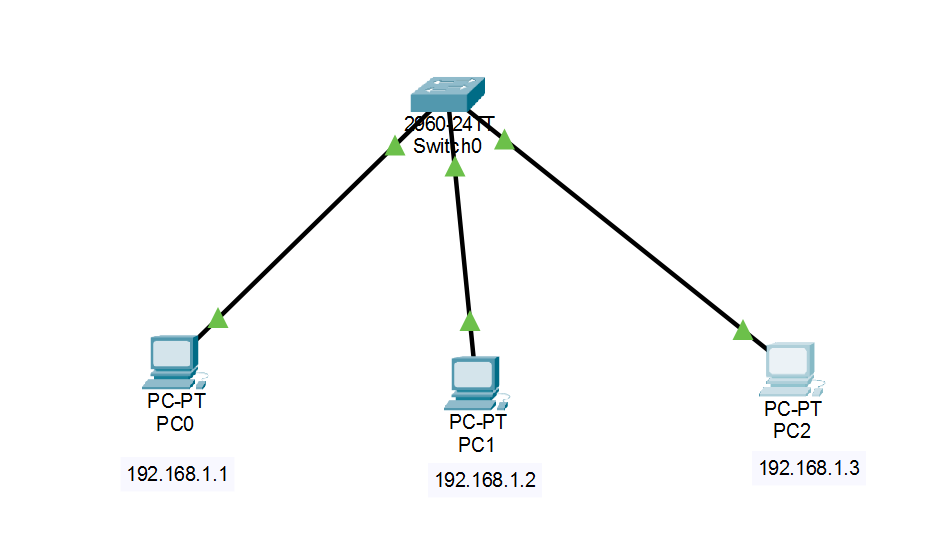
\includegraphics[width=0.7\textwidth]{images/9.1.png} 
    \caption{Wired LAN setup}
    \label{fig:network}
    \end{figure}
\subsubsection{IP Configuration:}
\begin{table}[h]
\centering
\begin{tabular}{|c|c|c|}
\hline
\textbf{Device} & \textbf{IP Address} & \textbf{Subnet Mask} \\
\hline
PC0 & 192.168.1.1 & 255.255.255.0 \\
PC1 & 192.168.1.2 & 255.255.255.0 \\
PC2 & 192.168.1.3 & 255.255.255.0 \\
\hline
\end{tabular}
\caption{IP Address Configuration}
\label{tab:ip_config}
\end{table}
    \begin{figure}[H]
    \centering
    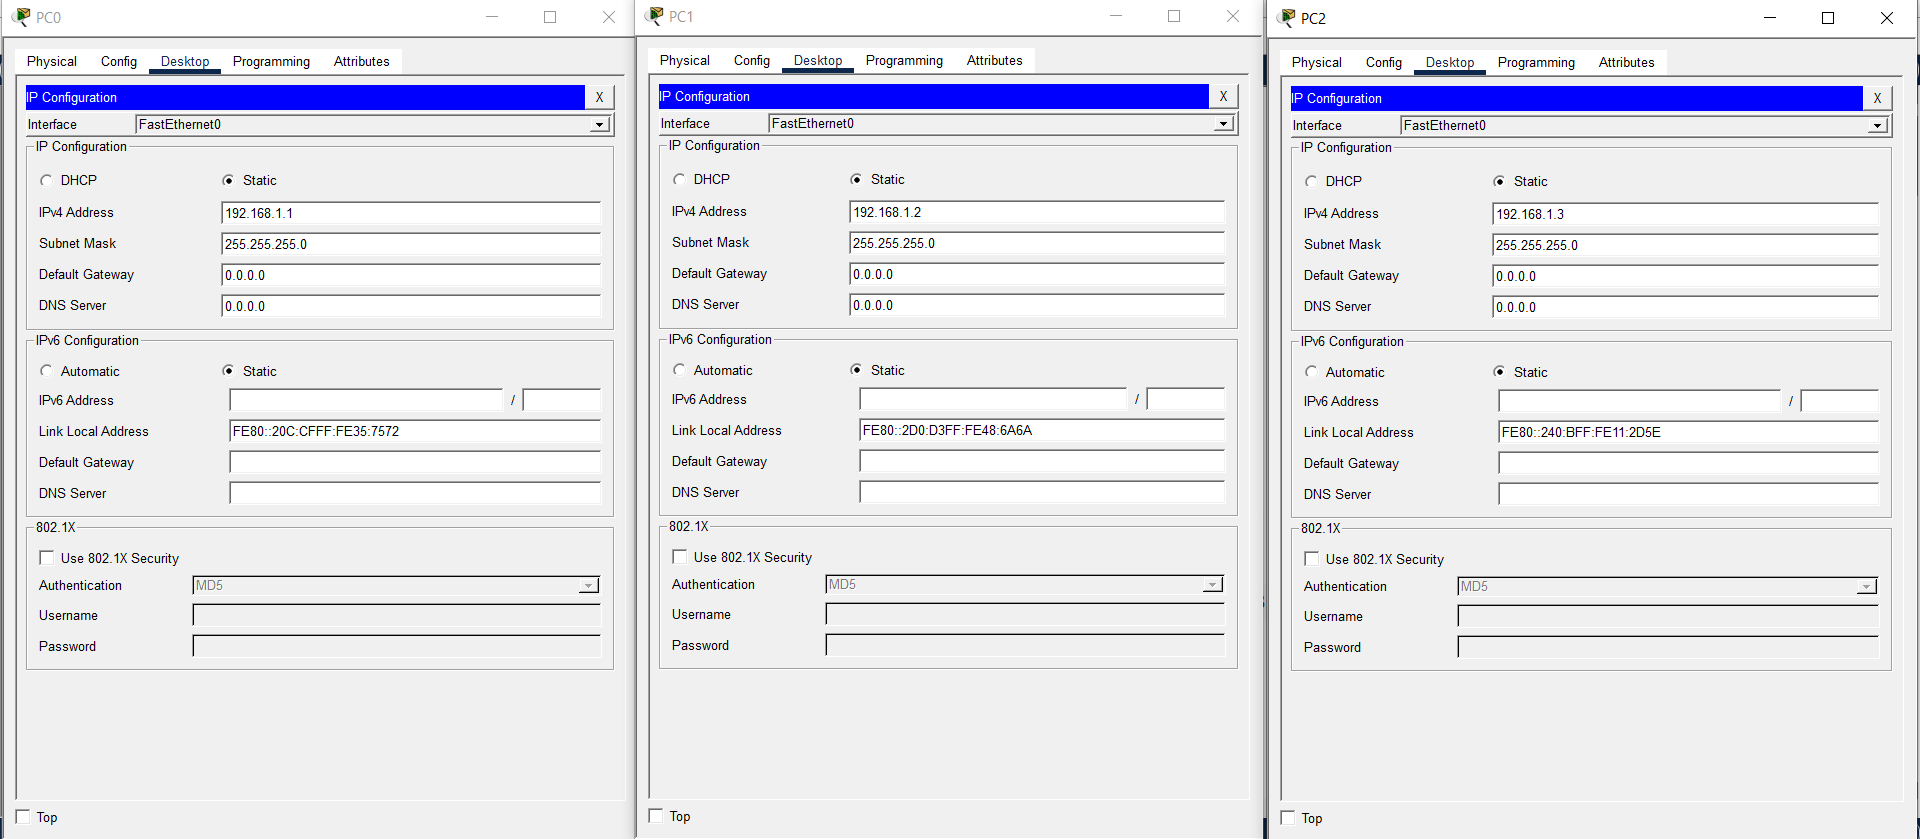
\includegraphics[width=1\textwidth]{images/9.2.png} 
    \caption{IP Address Configuration of PC0, PC1, PC2}
    \label{fig:network}
    \end{figure}
\subsubsection{Testing Connectivity:}
On PC0:
\begin{lstlisting}
ping 192.168.1.2
ping 192.168.1.3
\end{lstlisting}
    \begin{figure}[H]
    \centering
    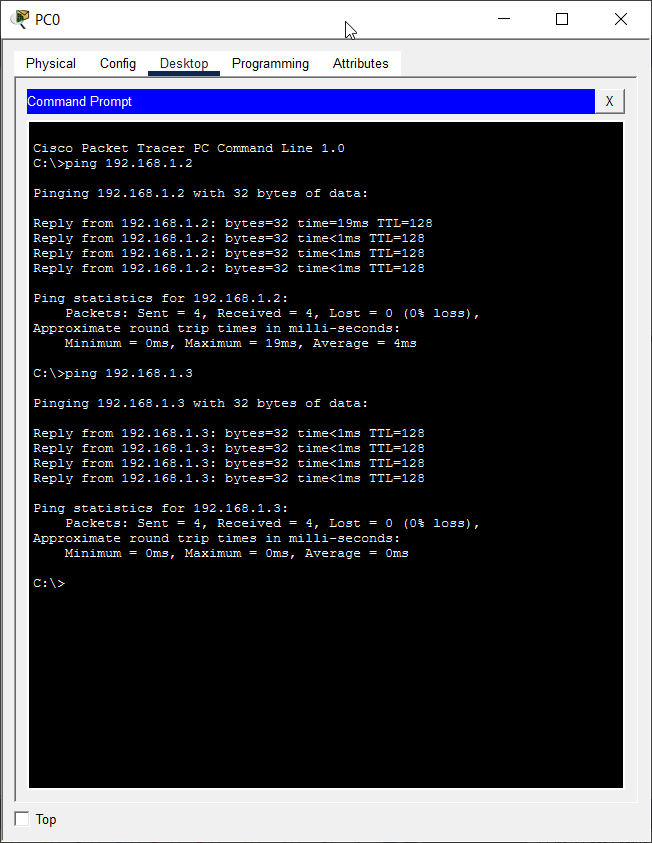
\includegraphics[width=1\textwidth]{images/9.3.png} 
    \caption{Wired LAN testing}
    \label{fig:network}
    \end{figure}
    
\subsection{Observation:}
\begin{itemize}
    \item PCs were successfully connected using Ethernet cables
    \item IP addresses were assigned correctly
    \item Ping command showed successful communication
    \item Wired LAN established successfully
\end{itemize}

\subsection{Viva Questions:}
\begin{enumerate}
    \item What is LAN?
    \item What is MAC address?
\end{enumerate}


% -------------------- EXPERIMENT - 10 --------------------
\newpage
\section{EXPERIMENT - 10}
\subsection{Title:}
Setup of Wireless LAN

\subsection{Aim/Objective:}
To configure and establish a Wireless Local Area Network (WLAN) using a wireless router and connect devices without cables.

\subsection{Theory:}
A Wireless LAN (WLAN) connects devices using radio waves instead of cables. Devices communicate through a Wireless Router or Access Point.
\begin{itemize}
    \item Uses SSID (network name) to identify the network
    \item Uses security (WPA2 password) to protect access
    \item Provides mobility and flexibility
\end{itemize}
Common examples: Wi-Fi in homes, colleges, offices

\subsection{Apparatus/Equipments/Softwares:}
\begin{itemize}
    \item Wireless Router
    \item Laptops / PCs (with wireless capability)
    \item Cisco Packet Tracer
\end{itemize}

\subsection{Procedure:}
\begin{enumerate}
    \item Open Cisco Packet Tracer
    
    \item Add:
    \begin{itemize}
        \item 1 Wireless Router (e.g., WRT300N)
        \item 2--3 Laptops
    \end{itemize}
    
    \item Click Wireless Router $\rightarrow$ GUI Tab
    
    \item Configure:
    \begin{itemize}
        \item SSID (e.g., MyWiFi)
        \item Security Mode $\rightarrow$ WPA2
        \item Password (e.g., 12345678)
    \end{itemize}
    
    \item On Laptop:
    \begin{itemize}
        \item Desktop $\rightarrow$ PC Wireless
        \item Select SSID (MyWiFi)
        \item Enter password
    \end{itemize}
    
    \item Assign IP (DHCP or manual)
    
    \item Test connectivity using \texttt{ping}
\end{enumerate}
    \begin{figure}[H]
    \centering
    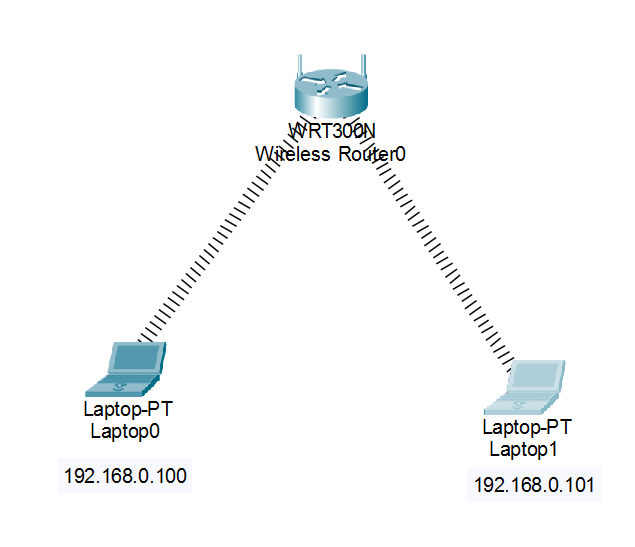
\includegraphics[width=0.5\textwidth]{images/10.1.png} 
    \caption{Wireless LAN setup}
    \label{fig:network}
    \end{figure}
    
    \begin{figure}[h]
    \centering
    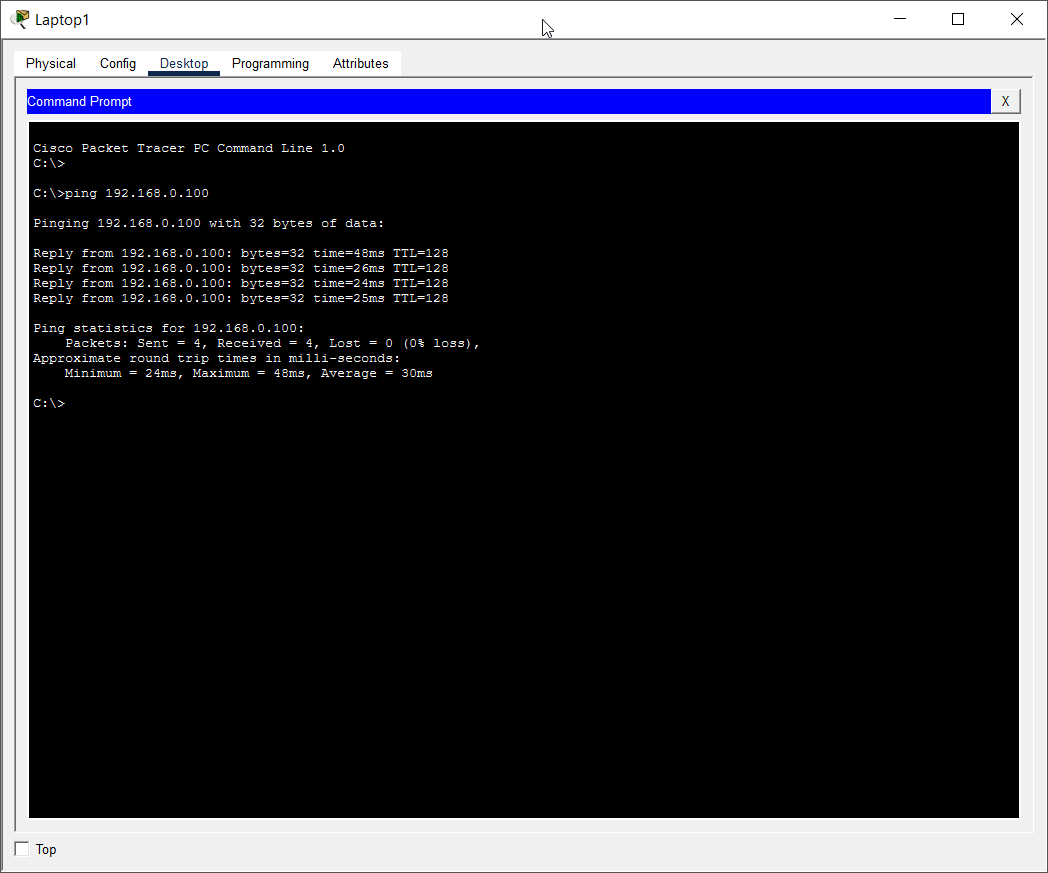
\includegraphics[width=1\textwidth]{images/10.2.png} 
    \caption{Wireless LAN testing}
    \label{fig:network}
    \end{figure}
    
\subsection{Observation:}
\begin{itemize}
    \item Wireless router configured successfully
    \item Devices connected using SSID and password
    \item Communication between devices verified using ping
    \item Wireless network established successfully
\end{itemize}

\subsection{Viva Questions:}
\begin{enumerate}
    \item What is SSID?
    \item Difference between wired and wireless LAN?
\end{enumerate}
    

\end{document}